% Manuscript for Computer Methods in Applied Mechanics and Engineering.
% Every number in the text, tables and figures comes from generated/ (written by
% scripts/make_cmame_material.py from the committed records); do not type numbers
% by hand. Build: latexmk -pdf main.tex (from this directory).
\documentclass[preprint,12pt]{elsarticle}

\usepackage[british]{babel}
\usepackage{amsmath,amssymb,amsthm}
\usepackage{graphicx}
\usepackage{booktabs}
\usepackage{array}
\usepackage{longtable}
\usepackage{xcolor}
\usepackage{tikz}
\usetikzlibrary{arrows.meta,positioning,fit}
\usepackage{microtype}
\usepackage[hidelinks,hypertexnames=false]{hyperref}
\usepackage[capitalise,nameinlink]{cleveref}
\biboptions{sort&compress}
\hypersetup{pdftitle={Training finite-element surrogates without solutions: the discrete
  potential energy as exact objective, metric and failure detector},
  pdfauthor={Ruifeng Cao, Xidan Song}}
\makeatletter
\g@addto@macro{\UrlBreaks}{\do\_\do\.}
\myfooterfont{\scriptsize\itshape}
% the first-page footer of elsarticle without the stray space after its box
\def\ps@pprintTitle{\let\@oddhead\@empty\let\@evenhead\@empty
  \def\@oddfoot{\@myfooterfont Preprint submitted to \@journal\hfill\@date}%
  \let\@evenfoot\@oddfoot}
\makeatother

% one-line footer, date as DD Month YYYY
\date{\number\day\space\ifcase\month\or January\or February\or March\or April\or May\or
  June\or July\or August\or September\or October\or November\or December\fi
  \space\number\year}

\newtheorem{lemma}{Lemma}
\newtheorem{proposition}{Proposition}
\newtheorem{corollary}{Corollary}
\theoremstyle{remark}
\newtheorem{remark}{Remark}
\crefname{lemma}{Lemma}{Lemmas}
\crefname{proposition}{Proposition}{Propositions}
\crefname{corollary}{Corollary}{Corollaries}
\crefname{remark}{Remark}{Remarks}

\newcommand{\norm}[1]{\lVert #1\rVert}
\newcommand{\gap}{\operatorname{gap}}
\newcommand{\vm}{\sigma_{\mathrm{vm}}}
\newcommand{\Ustar}{U^{\ast}}
\newcommand{\cstar}{c^{\ast}}
\newcommand{\R}{\mathbb{R}}
\newcommand{\pending}[1]{\par\smallskip\noindent\fbox{\parbox{\dimexpr\linewidth-2\fboxsep-2\fboxrule\relax}{\small\textbf{Pending.} #1}}\par\smallskip}

% generated by scripts/make_cmame_material.py from the records; do not edit
\newcommand{\numAmpFineCstar}{1.23}
\newcommand{\numAmpFineDisp}{0.258}
\newcommand{\numAmpFineDispC}{0.0832}
\newcommand{\numAmpFineGapMedian}{0.0911}
\newcommand{\numAmpFineGapMedianC}{0.0418}
\newcommand{\numAmpFineRedMax}{69\%}
\newcommand{\numAmpFineRedMin}{66\%}
\newcommand{\numAmpIdentity}{\ensuremath{2 \times 10^{-12}}}
\newcommand{\numAmpInCstar}{1.00}
\newcommand{\numAmpInDisp}{0.0300}
\newcommand{\numAmpInDispC}{0.0142}
\newcommand{\numAmpInGap}{0.00912}
\newcommand{\numAmpInGapC}{0.00740}
\newcommand{\numAmpRatioBoth}{5.9}
\newcommand{\numAmpRatioFineOnly}{2.8}
\newcommand{\numAmpRows}{4,608}
\newcommand{\numAuditItems}{22 of 22}
\newcommand{\numChebThree}{0.055}
\newcommand{\numChebTwo}{0.043}
\newcommand{\numCoarsenHigh}{2.5}
\newcommand{\numCoarsenHighCoarse}{0.174}
\newcommand{\numCoarsenHighFine}{0.198}
\newcommand{\numCoarsenHighReduction}{$-$23.7\%}
\newcommand{\numCoarsenHighWiden}{23.7\%}
\newcommand{\numCoarsenLow}{1.8}
\newcommand{\numCoarsenLowCoarse}{0.182}
\newcommand{\numCoarsenLowFine}{0.189}
\newcommand{\numCoarsenLowReduction}{$-$17.6\%}
\newcommand{\numCoarsenLowWiden}{17.6\%}
\newcommand{\numCondThree}{0.012}
\newcommand{\numCondTwo}{0.022}
\newcommand{\numCrossThree}{\ensuremath{7.43 \times 10^{-3}}}
\newcommand{\numCrossTwo}{\ensuremath{8.39 \times 10^{-3}}}
\newcommand{\numDfourteenAlpha}{\ensuremath{3.6 \times 10^{-4}}}
\newcommand{\numDfourteenDisp}{0.99964}
\newcommand{\numDfourteenGap}{0.99928}
\newcommand{\numDiagFixedMax}{0.22}
\newcommand{\numDiagFixedMin}{0.20}
\newcommand{\numDiagFixedSeeds}{six}
\newcommand{\numDiagScaledMax}{0.52}
\newcommand{\numDiagScaledMin}{0.22}
\newcommand{\numDiagSeeds}{six}
\newcommand{\numEOneBaseDisp}{0.0634}
\newcommand{\numEOneBaseGap}{0.0383}
\newcommand{\numEOneDeltaMax}{0.014}
\newcommand{\numEOneDeltaMin}{0.002}
\newcommand{\numEOneFloor}{0.02}
\newcommand{\numEtwoFineMax}{2.2}
\newcommand{\numEtwoFineMin}{1.8}
\newcommand{\numEtwoGapMax}{3.8}
\newcommand{\numEtwoGapMin}{2.8}
\newcommand{\numEtwoNodesFine}{41,367}
\newcommand{\numEtwoNodesIn}{12,318}
\newcommand{\numEtwoStepMax}{51}
\newcommand{\numEtwoStepMin}{38}
\newcommand{\numEtwoTransformerFineStep}{14.8}
\newcommand{\numFewFactorMax}{5.7}
\newcommand{\numFewFactorMin}{2.3}
\newcommand{\numFewSixteenDisp}{0.0531}
\newcommand{\numFewSixteenGap}{0.0702}
\newcommand{\numFewSixteenPeak}{0.389}
\newcommand{\numFewSixteenScratchDisp}{0.799}
\newcommand{\numFewSixteenVm}{0.166}
\newcommand{\numFewSixtyFourDisp}{0.0298}
\newcommand{\numFewSixtyFourGap}{0.0520}
\newcommand{\numFewSixtyFourPeak}{0.272}
\newcommand{\numFewSixtyFourScratchDisp}{0.193}
\newcommand{\numFewSixtyFourVm}{0.126}
\newcommand{\numFineFreeDisp}{0.258}
\newcommand{\numFineFreeGap}{0.306}
\newcommand{\numFineFreeVm}{0.305}
\newcommand{\numFineKill}{1.5}
\newcommand{\numFineKnnDisp}{0.401}
\newcommand{\numFineLabDisp}{0.257}
\newcommand{\numFineLabGap}{0.985}
\newcommand{\numFineLabVm}{0.537}
\newcommand{\numFineMgnDisp}{0.459}
\newcommand{\numFineMgnGap}{16.3}
\newcommand{\numFineMgnVm}{2.40}
\newcommand{\numFineRatio}{8.6}
\newcommand{\numFineWin}{1.25}
\newcommand{\numGOneFtDisp}{2.0\%}
\newcommand{\numGOneFtGap}{92.6\%}
\newcommand{\numGOneGapReduction}{78.7\%}
\newcommand{\numGOneRetired}{5.8\%}
\newcommand{\numGOneSanityMax}{6.1}
\newcommand{\numGOneSanityMin}{4.5}
\newcommand{\numGOneSanityTableSixteen}{2.4}
\newcommand{\numGOneVmReduction}{65.4\%}
\newcommand{\numGTwoAdvMin}{98.9\%}
\newcommand{\numGTwoFloor}{64}
\newcommand{\numGTwoParity}{$-$36.3\%}
\newcommand{\numGTwoSanityMax}{21.3}
\newcommand{\numGTwoSanitySixteen}{2.71}
\newcommand{\numGTwoSanitySixtyFour}{3.9}
\newcommand{\numGTwoSanityX}{3.0}
\newcommand{\numKappaTauTwo}{\ensuremath{1.5 \times 10^{-7}}}
\newcommand{\numKappaThreeHigh}{\ensuremath{5.2 \times 10^{5}}}
\newcommand{\numKappaThreeLow}{\ensuremath{2.9 \times 10^{4}}}
\newcommand{\numKappaTwoHigh}{\ensuremath{1.5 \times 10^{5}}}
\newcommand{\numKappaTwoLow}{\ensuremath{4.8 \times 10^{3}}}
\newcommand{\numKfiveEval}{64}
\newcommand{\numKfiveFiveGap}{0.0430}
\newcommand{\numKfiveFree}{242.5}
\newcommand{\numKfiveNaive}{261.3}
\newcommand{\numKfiveNaiveSaving}{$-$8.7\%}
\newcommand{\numKfiveSaving}{$-$0.9\%}
\newcommand{\numKfiveStartGap}{0.0722}
\newcommand{\numKfiveTol}{\ensuremath{10^{-6}}}
\newcommand{\numKfiveTwentyGap}{0.0260}
\newcommand{\numKfiveZero}{240.4}
\newcommand{\numKthreeBand}{3\%}
\newcommand{\numKthreeBaseRef}{0.201 $\pm$ 0.033}
\newcommand{\numKthreeBaseSeeds}{0.811, 6.99 and 1.66}
\newcommand{\numKthreeGain}{92.5\%}
\newcommand{\numKthreeOutside}{four}
\newcommand{\numKthreeWorse}{three}
\newcommand{\numMgnDispLowerMax}{92.6\%}
\newcommand{\numMgnDispLowerMin}{84.4\%}
\newcommand{\numMgnGapHigherMin}{99.2\%}
\newcommand{\numMgnLowerDispHigherVm}{685}
\newcommand{\numMgnPeakLowerMax}{29\%}
\newcommand{\numMgnPeakLowerMin}{17\%}
\newcommand{\numMgnVmHigher}{767}
\newcommand{\numModesPhrase}{$2 \times 10^{-15}$ in both dimensions}
\newcommand{\numModesThree}{\ensuremath{2 \times 10^{-15}}}
\newcommand{\numModesTwo}{\ensuremath{2 \times 10^{-15}}}
\newcommand{\numNodesFineMax}{71,749}
\newcommand{\numNodesFineMedian}{36,216}
\newcommand{\numNodesFineMin}{15,175}
\newcommand{\numNodesInMax}{17,692}
\newcommand{\numNodesInMedian}{5,617}
\newcommand{\numNodesInMin}{2,195}
\newcommand{\numPairThreeAncDisp}{81.2\%}
\newcommand{\numPairThreeAncGap}{99.7\%}
\newcommand{\numPairThreeAncPeak}{75.3\%}
\newcommand{\numPairThreeAncRecall}{95.7\%}
\newcommand{\numPairThreeAncVm}{99.7\%}
\newcommand{\numPairThreeLabDisp}{78.9\%}
\newcommand{\numPairThreeLabGap}{99.9\%}
\newcommand{\numPairThreeLabPeak}{87.4\%}
\newcommand{\numPairThreeLabRecall}{all}
\newcommand{\numPairThreeLabVm}{99.9\%}
\newcommand{\numPairTwoAncDisp}{36.2\%}
\newcommand{\numPairTwoAncGap}{91.8\%}
\newcommand{\numPairTwoAncPeak}{44.8\%}
\newcommand{\numPairTwoAncRecall}{76.4\%}
\newcommand{\numPairTwoAncVm}{75.1\%}
\newcommand{\numPairTwoLabDisp}{39.1\%}
\newcommand{\numPairTwoLabGap}{all}
\newcommand{\numPairTwoLabPeak}{63.2\%}
\newcommand{\numPairTwoLabRecall}{98.8\%}
\newcommand{\numPairTwoLabVm}{99.3\%}
\newcommand{\numParamsAux}{0.6}
\newcommand{\numParamsGraph}{3.9}
\newcommand{\numParamsTransformer}{6.7}
\newcommand{\numPilotDisp}{0.309}
\newcommand{\numPilotLimit}{0.90}
\newcommand{\numPremiseThree}{0.462}
\newcommand{\numPremiseTwo}{0.464}
\newcommand{\numRemeshFine}{1.27}
\newcommand{\numRemeshGeometries}{16}
\newcommand{\numRemeshInDev}{2\%}
\newcommand{\numRhoThree}{0.827}
\newcommand{\numRhoTwo}{0.730}
\newcommand{\numSqrtKappaMax}{723}
\newcommand{\numSqrtKappaMin}{69}
\newcommand{\numTauSqKappaTwo}{\ensuremath{6 \times 10^{-18}}}
\newcommand{\numTauSquared}{\ensuremath{10^{-12}}}
\newcommand{\numThreeAncDisp}{0.0470}
\newcommand{\numThreeAncGap}{0.116}
\newcommand{\numThreeAncGapMedian}{0.108}
\newcommand{\numThreeAncOverFreeGap}{12.7}
\newcommand{\numThreeAncPeak}{0.115}
\newcommand{\numThreeAncRecall}{0.730}
\newcommand{\numThreeAncVm}{0.128}
\newcommand{\numThreeAncWorse}{2}
\newcommand{\numThreeAncWorseTwoFiveSix}{4}
\newcommand{\numThreeEvalSolves}{2,048}
\newcommand{\numThreeFewSolves}{256}
\newcommand{\numThreeFreeDisp}{0.0300}
\newcommand{\numThreeFreeDispAdvantage}{36.3\%}
\newcommand{\numThreeFreeDispFour}{0.0300}
\newcommand{\numThreeFreeGap}{0.00912}
\newcommand{\numThreeFreeGapMedian}{0.00763}
\newcommand{\numThreeFreeLoadWorse}{1}
\newcommand{\numThreeFreeLoads}{3,072}
\newcommand{\numThreeFreeOverMgnDisp}{1.8}
\newcommand{\numThreeFreePeak}{0.0807}
\newcommand{\numThreeFreeRecall}{0.793}
\newcommand{\numThreeFreeVm}{0.0554}
\newcommand{\numThreeFreeWorse}{0}
\newcommand{\numThreeLabDisp}{0.0470}
\newcommand{\numThreeLabDispFour}{0.0470}
\newcommand{\numThreeLabGap}{31.2}
\newcommand{\numThreeLabGapMedian}{0.252}
\newcommand{\numThreeLabGapMs}{31.2 $\pm$ 53.5}
\newcommand{\numThreeLabGapSeeds}{0.297, 93.0, 0.365}
\newcommand{\numThreeLabPeak}{0.784}
\newcommand{\numThreeLabRecall}{0.619}
\newcommand{\numThreeLabVm}{0.370}
\newcommand{\numThreeLabWorse}{18}
\newcommand{\numThreeLabWorseTwoFiveSix}{132}
\newcommand{\numThreeLabWorst}{23,727}
\newcommand{\numThreeLabWorstSeed}{1}
\newcommand{\numThreeMedianRatioMax}{33}
\newcommand{\numThreeMedianRatioMin}{14}
\newcommand{\numThreeMgnDisp}{0.0168}
\newcommand{\numThreeMgnGap}{0.447}
\newcommand{\numThreeMgnGapMedian}{0.208}
\newcommand{\numThreeMgnOverFreePeak}{6.0}
\newcommand{\numThreeMgnOverFreeVm}{5.3}
\newcommand{\numThreeMgnPeak}{0.488}
\newcommand{\numThreeMgnRecall}{0.679}
\newcommand{\numThreeMgnVm}{0.296}
\newcommand{\numThreeMgnWorse}{28}
\newcommand{\numThreePairs}{768}
\newcommand{\numThreeSolves}{6,400}
\newcommand{\numThreeTrainSolves}{4,096}
\newcommand{\numThreeVal}{256}
\newcommand{\numTimeBottleneckSeedMax}{2.5}
\newcommand{\numTimeBottleneckSeedMin}{2.5}
\newcommand{\numTimeBottleneckSpeedup}{11}
\newcommand{\numTimeThreeSeed}{27.3}
\newcommand{\numTimeTwoParallel}{2 h 58 min}
\newcommand{\numTwoAdvMax}{98.7\%}
\newcommand{\numTwoAdvMin}{80.4\%}
\newcommand{\numTwoAncDisp}{0.161}
\newcommand{\numTwoAncGap}{0.166}
\newcommand{\numTwoAncGapMedian}{0.0709}
\newcommand{\numTwoAncPeak}{0.246}
\newcommand{\numTwoAncRecall}{0.708}
\newcommand{\numTwoAncSixteenSeeds}{0.225, 0.458, 0.546}
\newcommand{\numTwoAncVm}{0.257}
\newcommand{\numTwoAncWorse}{14}
\newcommand{\numTwoFreeDisp}{0.166}
\newcommand{\numTwoFreeDispExcess}{+3.6\%}
\newcommand{\numTwoFreeDispExcessAbs}{3.6\%}
\newcommand{\numTwoFreeDispFour}{0.1658}
\newcommand{\numTwoFreeGap}{0.0817}
\newcommand{\numTwoFreeGapMedian}{0.0493}
\newcommand{\numTwoFreePeak}{0.228}
\newcommand{\numTwoFreeRecall}{0.739}
\newcommand{\numTwoFreeVm}{0.210}
\newcommand{\numTwoFreeWorse}{3}
\newcommand{\numTwoFtDisp}{0.166}
\newcommand{\numTwoFtGap}{0.236}
\newcommand{\numTwoFtGapMedian}{0.156}
\newcommand{\numTwoFtPeak}{0.301}
\newcommand{\numTwoFtRecall}{0.645}
\newcommand{\numTwoFtVm}{0.336}
\newcommand{\numTwoFtWorse}{21}
\newcommand{\numTwoGapSpread}{31}
\newcommand{\numTwoLabDisp}{0.160}
\newcommand{\numTwoLabDispFour}{0.1600}
\newcommand{\numTwoLabGap}{0.418}
\newcommand{\numTwoLabGapMedian}{0.274}
\newcommand{\numTwoLabOverFreeGap}{5.1}
\newcommand{\numTwoLabPeak}{0.334}
\newcommand{\numTwoLabRecall}{0.584}
\newcommand{\numTwoLabVm}{0.433}
\newcommand{\numTwoLabWorse}{52}
\newcommand{\numTwoMgnDisp}{0.167}
\newcommand{\numTwoMgnGap}{2.57}
\newcommand{\numTwoMgnGapMedian}{1.35}
\newcommand{\numTwoMgnPeak}{1.32}
\newcommand{\numTwoMgnRecall}{0.322}
\newcommand{\numTwoMgnVm}{1.10}
\newcommand{\numTwoMgnWorse}{481}
\newcommand{\numTwoPairs}{768}
\newcommand{\numTwoRuns}{nine}
\newcommand{\numTwoRunsDisp}{0.1658 $\pm$ 0.0023}
\newcommand{\numTwoRunsGap}{0.0820 $\pm$ 0.0026}
\newcommand{\numTwoSolves}{7,168}
\newcommand{\numTwoSolvesOffline}{5,120}
\newcommand{\numTwoSolvesRun}{2,048}
\newcommand{\numTwoVal}{256}
\newcommand{\numWarmFractionSeven}{15\%}
\newcommand{\numWarmFractionSeventeen}{6\%}
\newcommand{\numWarmFractionTwelve}{9\%}
\newcommand{\numWithinThree}{\ensuremath{6.76 \times 10^{-2}}}
\newcommand{\numWithinTwo}{\ensuremath{7.56 \times 10^{-2}}}
\newcommand{\numWorstFreeDisp}{0.071}
\newcommand{\numWorstFreeGap}{0.0349}
\newcommand{\numWorstFreeVm}{0.10}
\newcommand{\numWorstIndex}{107}
\newcommand{\numWorstLabDisp}{0.032}
\newcommand{\numWorstLabGap}{2.90}
\newcommand{\numWorstLabVm}{0.73}
\newcommand{\numWorstMgnDisp}{0.033}
\newcommand{\numWorstMgnGap}{27.0}
\newcommand{\numWorstMgnVm}{2.4}
\newcommand{\numWorstSeedLabDisp}{0.55}
\newcommand{\numWorstSeedLabPeak}{361}
\newcommand{\numWorstSeedLabVm}{65}


\journal{Computer Methods in Applied Mechanics and Engineering}

\begin{document}

\begin{frontmatter}

\title{Training finite-element surrogates without solutions: the discrete potential
energy as exact objective, metric and failure detector}

\author[man]{Ruifeng Cao\corref{cor1}}
\ead{ruifeng.cao@manchester.ac.uk}
\author[whu]{Xidan Song\corref{cor1}}
\ead{liuqingdamafen@whu.edu.cn}
\cortext[cor1]{Corresponding authors.}

\affiliation[man]{organization={School of Engineering, The University of Manchester},
  addressline={Oxford Road}, city={Manchester}, postcode={M13~9PL},
  country={United Kingdom}}
\affiliation[whu]{organization={School of Computer Science, Wuhan University},
  addressline={299 Bayi Road, Wuchang District}, city={Wuhan}, postcode={430072},
  country={China}}

\begin{abstract}
Supervised training of a finite-element surrogate requires a full solve for every training
example, the very cost the surrogate should remove. For linear elastostatics we train on
the assembled discrete potential energy instead. Minimising it is exactly supervised
regression in the stiffness norm, which measures the strain energy of the error, so the
surrogate learns from a weighted mean-square stress error without solving any example. In pre-registered comparisons on three-dimensional tetrahedral
meshes, a transformer trained on the energy alone was more accurate, on every metric,
than the same network trained on the solutions of the same instances. A supervised graph
network had smaller displacement errors on most instances but larger stress-field errors
on almost all: displacement error ranked the two in the opposite order to stress error.
Every supervised network there returned some predictions worse than the zero field in the
energy norm, failures the energy detects without reference solutions. In two dimensions
the label-free transformer had a larger displacement error than its supervised
counterpart but smaller stress errors; trained on the stiffness-norm error instead, with
the same labels, the counterpart halved its von Mises error, as pre-registered, and its
errors lay in softer stiffness eigenmodes, as measured afterwards: with the labels fixed,
the norm of the loss decided the stress accuracy. No network transferred to a
substantially finer three-dimensional mesh without retraining; a post hoc, closed-form,
label-free rescaling removed most of the label-free network's error there. The discrete
energy thus serves as training objective, evaluation metric and failure detector.

\end{abstract}

\begin{keyword}
finite element method \sep surrogate modelling \sep label-free training \sep
minimum total potential energy \sep energy norm \sep pre-registration
\end{keyword}

\end{frontmatter}

\section{Introduction}\label{sec:intro}

% DRAFT: to be revised after the full texts of [Wang2026PretrainFEM], [Sun2026FEVessel]
% and [MonteiroFernandes2025] have been read (outline v3, Sec. 7).

Neural surrogates of finite-element analyses are trained to return, in one network
evaluation, the field that an assembly and solve would return, so that design studies,
optimisation and uncertainty quantification can query many configurations cheaply
\cite{Pfaff2021,Lu2021DeepONet,Li2021FNO,He2024GeomDeepONet,Zeng2025PCNO,Liu2026GINOT}.
Most are trained by supervised regression on reference solutions. Each reference
solution is a full solve of the system that the surrogate is meant to replace, so the
training set costs, before the surrogate has made its first prediction, as many solves as
it has instances and load cases; every extension of scope, to a new geometry family, load
regime or mesh resolution, costs more.

For linear elastostatics there is a training signal that needs no solve. The
finite-element solution minimises the assembled discrete potential energy
$\Pi_h(u)=\tfrac12u^{\top}Ku-F^{\top}u$, whose stiffness matrix $K$ and load vector $F$
every finite-element code assembles before it solves; evaluating $\Pi_h$ at a prediction
$u$ costs one sparse matrix-vector product. The energy of a prediction exceeds that of
the solution $\Ustar$ by half the squared stiffness-norm error,
$\Pi_h(u)-\Pi_h(\Ustar)=\tfrac12\norm{u-\Ustar}_K^2$, a classical identity of the
energy-norm theory of finite elements \cite{Ciarlet1978}, and this half squared norm is the
strain energy of the error's stress field. Minimising the energy over a set of training
instances is therefore exactly supervised regression in the stiffness norm, with the same
gradients at every point: a surrogate trained on the energy learns from a weighted
mean-square stress error, and no training instance is ever solved.

Energy minimisation as a training principle is not new. The deep Ritz method
\cite{EYu2018} and the deep energy method \cite{Samaniego2020} minimise a continuous energy
over neural trial functions, and later work trains operators and mesh-based networks
without labels, with residual or energy losses
\cite{Xu2024VOL,Eshaghi2025VINO,Lee2025FEONet,Dalton2023,Wurth2024,Wang2026PretrainFEM}
(\cref{sec:related}). That the energy ranks candidate fields is the Ritz minimum principle
itself. This paper adds two things for neural surrogates. The first is the systematic use
of that principle to evaluate and screen their predictions without reference solutions: an
exact link from the energy to the stress error, a test that tells whether a prediction is
worse than the zero field, and a closed-form rescaling that guarantees it is not. The second
is a controlled test of what label-free training buys: the same network trained on the same
instances with and without their solutions, under criteria fixed before the runs, with the
criteria that failed reported alongside those that were met. By the identity above, the
test compares two losses, the stiffness-norm error, which needs no solve, and the usual
relative displacement error, which does; the labels add no information that $K$ and $F$ do
not already carry. The paper extends a companion note \cite{CaoSong2026}, which stated the
exactness identity, the conditioning bounds and their executable checks.

The contributions are as follows.
\begin{enumerate}
\item Theory (\cref{sec:theory}). The label-free energy objective is supervised
stiffness-norm regression (\cref{lem:exact,cor:training}); for isotropic elasticity the
energy gap is a compliance-weighted mean-square error of the stress field and bounds the
error of the von Mises field (\cref{prop:stress}). Displacement and energy-norm errors can
rank two predictions in opposite orders only when their displacement errors differ by less
than the square root of the condition number of $K$, and then they can
(\cref{rem:rank}). The sign of $\Pi_h(u)$ tells, for each load case, whether a prediction is
worse than the zero field (\cref{cor:zero}), and the two terms of $\Pi_h(u)$ give a
rescaling after which it is not (\cref{prop:amp}). Under the classical Chebyshev bound, a
warm start lowers the iteration bound of conjugate gradients by a fraction that depends
only on the prediction's relative energy gap and the target tolerance (\cref{cor:warm}).
\item Experiments (\cref{sec:results2d,sec:results3d}). On three-dimensional tetrahedral
meshes, a transformer trained on the energy alone was more accurate on all five metrics,
in every seed, than the same transformer trained on the solutions of the same 1,024
instances. A graph network trained on those solutions had lower displacement errors than
the label-free transformer on most instances but higher stress errors on almost all of
them, so that displacement error ranked the two in the opposite order to stress error.
Every supervised network returned some in-band predictions worse than the zero field; the
label-free network returned none, averaged over each instance's load cases, and
\numThreeFreeLoadWorse{} in \numThreeFreeLoads{} load cases taken singly. In two dimensions, the label-free network's
displacement error was \numTwoFreeDispExcessAbs{} larger than the supervised network's, and
it was more accurate on every other metric.
\item Negative results (\cref{sec:results2d,sec:transfer,sec:cost}). In two dimensions,
conjugate gradients started from a label-free prediction did not need fewer iterations to a
tight residual tolerance than from zero. No network transferred to a three-dimensional mesh
about twice as fine without retraining; a closed-form rescaling applied after the fact
removed about two-thirds of the label-free network's displacement error there.
\item Cost (\cref{sec:cost}). The label-free network was trained without a single solve;
in three dimensions the supervised networks' 1,024 labelled training instances took
\numThreeTrainSolves{} solves, and evaluating any method on the in-band and fine-mesh
validation sets took a further \numThreeEvalSolves{}.
\end{enumerate}

We do not claim that a surrogate is faster than solving a linear elastostatic problem:
sparse direct and iterative solvers are fast at the sizes studied here
(\cref{sec:cost}). Linear elastostatics is the test bed on which the exactness of the
objective can be proved and the comparison with supervision kept narrow: the same network,
the same instances and the same schedule, with only the loss and its learning rate
differing. The interest of label-free training lies where solves are expensive and labels
scarce, for example in nonlinear and time-dependent problems whose implicit steps are again
energy minimisations (\cref{sec:discussion}).

\Cref{sec:related} reviews related work, \cref{sec:theory} the theory and
\cref{sec:methods} the problems, networks and protocol. \Cref{sec:results2d,sec:results3d}
report the two- and three-dimensional comparisons, \cref{sec:transfer} the transfer to a
finer mesh and \cref{sec:cost} the cost. \Cref{sec:discussion} discusses the results and
their limits. \ref{app:prereg} lists every pre-registered criterion with its outcome and
the deviations from the plans, \ref{app:e1} a negative result on latent regularisation
and \ref{app:repro} how every number is reproduced from the records.

\section{Related work}\label{sec:related}

% DRAFT: every characterisation below is to be checked against the full text of the cited
% work before submission; three works are flagged in the text.

\paragraph{Energy and variational training of neural solvers}
The deep Ritz method \cite{EYu2018} minimises the continuous energy of a variational
problem over neural trial functions, and the deep energy method \cite{Samaniego2020}
brought the idea to computational mechanics. Later work treated essential boundary
conditions \cite{LiaoMing2021} and showed that the numerical quadrature which evaluates the
continuous functional contributes an error of its own, which enters the objective itself
\cite{LiuCaiRamani2023}. Variational and weak-form losses followed: hp-VPINNs
\cite{Kharazmi2021}, conservative energy methods on subdomains \cite{Wang2022CENN},
Kolmogorov--Arnold-informed networks \cite{Wang2025KINN} and energy-based phase-field
fracture \cite{Manav2024}. Robust variational physics-informed networks \cite{Rojas2024}
and the deep Fourier residual method \cite{Taylor2023DFR,Taylor2024} construct losses
equivalent to the energy norm of the error by measuring the residual in a dual norm.
\Cref{lem:exact} and \cref{rem:dual} below are the exact algebraic counterpart of that
equivalence on the assembled system: no quadrature error and no equivalence constants,
because the inverse in the dual norm cancels.

\paragraph{Label-free surrogates and operators}
Variational operator learning \cite{Xu2024VOL} trains operators on the finite-element
system, evaluated matrix-free, and uses the gradient identity of
\cref{lem:exact} as a computational device; its loss is the Euclidean norm of the
residual, or a regression on provisional labels produced by a few conjugate-gradient
iterations. The variational physics-informed neural operator \cite{Eshaghi2025VINO}
evaluates the continuous functional analytically on its own bilinear discretisation over
uniform grids. Other label-free approaches build on the finite-element residual or weak
form \cite{Lee2025FEONet,Uriarte2022,Gao2022,Goswami2022}. Closest to the present work are
graph networks on finite-element meshes trained by minimising the potential energy
\cite{Dalton2023}, physics-informed MeshGraphNets trained without data for non-stationary
and nonlinear problems \cite{Wurth2024}, a physics-informed three-dimensional surrogate for
elastic fields in polycrystals \cite{MonteiroFernandes2025}, and the pretrain finite
element method \cite{Wang2026PretrainFEM}, which pretrains a physics-informed neural
operator without labels and uses its prediction to warm-start the finite-element solver;
its authors report speed-ups of up to an order of magnitude in the warm-start stage. A
follow-up applies that approach to three-dimensional pressure vessels
\cite{Sun2026FEVessel}. Some of these works compare label-free with data-driven training
\cite{Wurth2024,MonteiroFernandes2025}. We are not aware of a comparison of the same
network trained on the same instances with and without their solutions under criteria
fixed in advance, nor of the use of the energy to evaluate and screen surrogate predictions;
both statements, and the characterisations of this paragraph, are to be confirmed against
the full texts of \cite{MonteiroFernandes2025,Wang2026PretrainFEM,Sun2026FEVessel} before
submission.

\paragraph{Supervised mesh surrogates}
MeshGraphNets \cite{Pfaff2021} learn mesh-based simulation by message passing; operator
networks such as DeepONet \cite{Lu2021DeepONet} and the Fourier neural operator
\cite{Li2021FNO} learn maps between function spaces; and point-cloud and
geometry-aware operators handle variable three-dimensional geometries
\cite{He2024GeomDeepONet,Zeng2025PCNO,Liu2026GINOT}. Graph networks have also emulated
cardiac mechanics \cite{Dalton2022}. These surrogates are typically trained and evaluated
with relative $L^2$ errors of the predicted fields. \Cref{rem:rank} and
\cref{sec:results3d} show that the displacement error can rank surrogates in the opposite
order to their stress errors.

\paragraph{Solvers, warm starts and conditioning}
Neural predictions have been used as initial iterates of iterative solvers
\cite{Wang2026PretrainFEM,Eshaghi2026NOWS} and inside hybrid iterative schemes
\cite{Lee2025MetaSolver}. \Cref{cor:warm} bounds how far a warm start can lower the
iteration bound of conjugate gradients, and \cref{sec:results2d:decisions} reports a
pre-registered test in which a warm start saved nothing at a tight tolerance. The training difficulty of
residual-based physics losses has been traced to operator conditioning: descent on a
squared residual is governed by an operator whose condition number is the square of the
original one \cite{DeRyck2024}; the energy objective avoids the squaring
(\cref{rem:dual}).

\paragraph{Fair comparison and pre-registration}
Weak baselines and selective reporting have led to over-optimism in machine learning for
fluid-related partial differential equations \cite{McGreivy2024}, and a comprehensive and
fair comparison of two neural operators needed common data and protocols
\cite{Lu2022Fair}. Pre-registration, the recording of hypotheses, analyses and decision
criteria in a dated document before the data are seen, is established in other sciences as
a guard against these biases \cite{Nosek2018}. Each run whose results decide a claim of
this paper was pre-registered, with executable checks that refuse a run whose configuration
differs from the registered one, and every criterion fixed in advance for these runs is
reported with its outcome (\cref{sec:methods:prereg}, \ref{app:prereg}).

\section{Theory}\label{sec:theory}

This section collects the identities on which the method and its evaluation rest.
\Cref{lem:exact,lem:cond}, \cref{cor:modes}, \cref{rem:dual} and \cref{prop:sep} of
\ref{app:e1} are restated, with proofs, from the companion note \cite{CaoSong2026}, and
\eqref{eq:cheb} is the classical Chebyshev bound of conjugate gradients \cite{Saad2003}; the other
statements are added here. All are elementary consequences of the energy-norm algebra of
symmetric positive definite systems \cite{Ciarlet1978,Saad2003}. What they provide is an
exact account of what label-free training optimises, of how its results should be measured,
and of what the energy of a prediction reveals without a reference solution. Each statement
with numerical content is implemented as an executable check (\cref{sec:theory:checks}).

\subsection{Discrete setting}\label{sec:theory:setting}

Consider a linear elastostatic problem on a domain $\Omega\subset\R^{d}$, $d\in\{2,3\}$,
discretised by conforming finite elements, with homogeneous Dirichlet conditions on part
of the boundary. After the constrained degrees of freedom are eliminated, the $n$ free
nodal displacements of the finite-element solution $\Ustar\in\R^{n}$ satisfy
\begin{equation}
K\Ustar = F,
\label{eq:system}
\end{equation}
where $K\in\R^{n\times n}$ is the stiffness matrix restricted to the free degrees of
freedom and $F\in\R^{n}$, $F\neq0$, the load vector. We call $\Ustar$ the reference
solution; with sufficient Dirichlet constraints, $K$ is symmetric positive definite. The
discrete potential energy of a vector $u\in\R^{n}$ is
\begin{equation}
\Pi_h(u) = \tfrac12\,u^{\top}Ku - F^{\top}u ,
\label{eq:energy}
\end{equation}
and the stiffness norm, or energy norm, is $\norm{v}_K=(v^{\top}Kv)^{1/2}$ for
$v\in\R^{n}$. For a prediction $u$ with error $e=u-\Ustar$ we call
$\gap(u)=\Pi_h(u)-\Pi_h(\Ustar)$ its energy gap and
\begin{equation}
g(u) = \frac{\norm{u-\Ustar}_K^{2}}{\norm{\Ustar}_K^{2}}
\label{eq:relgap}
\end{equation}
its relative energy gap. Substituting \eqref{eq:system} into \eqref{eq:energy} gives
$\Pi_h(\Ustar)=-\tfrac12\norm{\Ustar}_K^2$, so the zero field has $g(0)=1$. The smallest
and largest eigenvalues of $K$ are $\lambda_{\min}$ and $\lambda_{\max}$, and
$\kappa=\lambda_{\max}/\lambda_{\min}$ is its spectral condition number. Evaluating
$\Pi_h(u)$ requires $K$ and $F$, which every finite-element code assembles before solving,
and one sparse matrix-vector product; it does not require $\Ustar$. The energy gap and
$g$ do require $\Ustar$: in this paper they are evaluation quantities, computed on
validation instances only.

\subsection{Label-free training is stiffness-norm regression}\label{sec:theory:exact}

\begin{lemma}[Exactness]\label{lem:exact}
For every $u\in\R^{n}$,
\begin{equation}
\Pi_h(u)-\Pi_h(\Ustar) = \tfrac12\norm{u-\Ustar}_K^{2}
\qquad\text{and}\qquad
\nabla\Pi_h(u) = K(u-\Ustar).
\label{eq:exact}
\end{equation}
\end{lemma}

\begin{proof}
Expanding $\tfrac12\norm{u-\Ustar}_K^2=\tfrac12u^{\top}Ku-u^{\top}K\Ustar
+\tfrac12\Ustar{}^{\top}K\Ustar$ and using $K\Ustar=F$ gives
$\tfrac12\norm{u-\Ustar}_K^2=\Pi_h(u)+\tfrac12\norm{\Ustar}_K^2=\Pi_h(u)-\Pi_h(\Ustar)$.
Differentiating \eqref{eq:energy} gives $\nabla\Pi_h(u)=Ku-F=K(u-\Ustar)$.
\end{proof}

Hence $g(u)=\gap(u)/\lvert\Pi_h(\Ustar)\rvert$: the relative energy gap is the ratio of the
strain energy of the error to that of the solution. A surrogate is trained on many
instances. Let instance $i\in\{1,\dots,N\}$ have stiffness matrix $K_i$ and $L$ load
vectors $F_{ij}$, $j\in\{1,\dots,L\}$, with solutions $\Ustar_{ij}=K_i^{-1}F_{ij}$ and
energies $\Pi_{ij}(u)=\tfrac12u^{\top}K_iu-F_{ij}^{\top}u$, and let $u_{ij}(\theta)$ be the
prediction of a network with parameters $\theta$.

\begin{corollary}[Training objective]\label{cor:training}
The label-free objective satisfies
\begin{equation}
\mathcal{L}_{\Pi}(\theta) = \frac{1}{NL}\sum_{i=1}^{N}\sum_{j=1}^{L}\Pi_{ij}\bigl(u_{ij}(\theta)\bigr)
= \frac{1}{NL}\sum_{i=1}^{N}\sum_{j=1}^{L}\tfrac12\norm{u_{ij}(\theta)-\Ustar_{ij}}_{K_i}^{2}
+ \Pi^{\ast},
\label{eq:training}
\end{equation}
where $\Pi^{\ast}=\frac{1}{NL}\sum_{i,j}\Pi_{ij}(\Ustar_{ij})$ does not depend on $\theta$.
Minimising $\mathcal{L}_\Pi$ is therefore supervised regression in the stiffness norm: the
two objectives have the same minimisers and the same gradient with respect to $\theta$ at
every $\theta$, yet $\mathcal{L}_\Pi$ is evaluated without any $\Ustar_{ij}$.
\end{corollary}

\begin{proof}
Apply \cref{lem:exact} to each term; the chain rule carries the equality of gradients
from $u_{ij}$ to $\theta$.
\end{proof}

The regression in \eqref{eq:training} sums squared energy-norm errors without normalising
them, so instances whose solutions carry more strain energy weigh more. Normalising each
term by $\lvert\Pi_{ij}(\Ustar_{ij})\rvert$ would require the solutions; the label-free
objective cannot do it.

\begin{remark}[Dual norm]\label{rem:dual}
With the residual $r(u)=F-Ku=-Ke$, \cref{lem:exact} reads
$\gap(u)=\tfrac12\,r(u)^{\top}K^{-1}r(u)$: the energy gap is half the squared residual
measured in the norm induced by $K^{-1}$, the norm in which a small residual means an
accurate solution. The inverse cancels algebraically in $\Pi_h$, so the objective needs
neither a solve nor a preconditioner. A Euclidean residual loss, by contrast, is
$\norm{r(u)}_2^2=e^{\top}K^{2}e$, a regression in the norm of $K^2$, whose condition
number is $\kappa^2$ \cite{DeRyck2024}.
\end{remark}

\subsection{The energy gap measures the stress error}\label{sec:theory:stress}

Let $v_h$ denote the finite-element displacement field of a vector $v\in\R^n$, extended by
zero on the constrained degrees of freedom, $\varepsilon(v_h)$ its strain,
$\sigma(v_h)=\mathbb{C}:\varepsilon(v_h)$ its stress for the fourth-order elasticity
tensor $\mathbb{C}$, $s=\sigma-\tfrac13(\operatorname{tr}\sigma)I$ the deviatoric stress,
$p=\tfrac13\operatorname{tr}\sigma$ the mean stress and $\vm(\sigma)=(\tfrac32\,s:s)^{1/2}$
the von Mises stress of a stress tensor $\sigma$; we write $\vm(v_h)$ and $p(v_h)$ for the
fields $\vm(\sigma(v_h))$ and $p(\sigma(v_h))$. For a homogeneous isotropic material with Young's modulus $E$ and Poisson's
ratio $\nu$, $G=E/(2(1+\nu))$ is the shear modulus and $B=E/(3(1-2\nu))$ the bulk modulus.

\begin{proposition}[Energy gap and stress error]\label{prop:stress}
Let the material be homogeneous and isotropic and the stiffness matrix be integrated
exactly, as it is for linear elements. For every $v\in\R^{n}$,
\begin{equation}
\norm{v}_K^{2} = \int_{\Omega}\sigma(v_h):\mathbb{C}^{-1}:\sigma(v_h)\,\mathrm{d}\Omega
= \int_{\Omega}\Bigl(\frac{\vm(v_h)^{2}}{3G}+\frac{p(v_h)^{2}}{B}\Bigr)\mathrm{d}\Omega .
\label{eq:stressnorm}
\end{equation}
Consequently, for a prediction $u$ with error $e=u-\Ustar$,
\begin{equation}
\gap(u) = \frac12\int_{\Omega}\bigl(\sigma(u_h)-\sigma(\Ustar_h)\bigr):\mathbb{C}^{-1}:
\bigl(\sigma(u_h)-\sigma(\Ustar_h)\bigr)\,\mathrm{d}\Omega ,
\label{eq:gapstress}
\end{equation}
and the von Mises fields of $u$ and $\Ustar$ satisfy
\begin{gather}
\bigl\lVert\vm(u_h)-\vm(\Ustar_h)\bigr\rVert_{L^2(\Omega)}^{2}\le 3G\,\norm{u-\Ustar}_K^{2},
\label{eq:vmbound}\\
\frac{\lVert\vm(u_h)-\vm(\Ustar_h)\rVert_{L^2(\Omega)}^{2}}{\lVert\vm(\Ustar_h)\rVert_{L^2(\Omega)}^{2}}
\le (1+\gamma^{\ast})\,g(u),
\label{eq:vmboundrel}
\end{gather}
where $\gamma^{\ast}=3G\lVert p(\Ustar_h)\rVert_{L^2(\Omega)}^2/
(B\lVert\vm(\Ustar_h)\rVert_{L^2(\Omega)}^2)$, defined when $\vm(\Ustar_h)\neq0$, is the
ratio of the volumetric to the deviatoric strain energy of the solution. In plane stress
the same statements hold for the plane stress state, with the three-dimensional moduli $G$
and $B$.
\end{proposition}

\begin{proof}
For a conforming discretisation with exactly integrated stiffness,
\begin{equation*}
v^{\top}Kv=\int_\Omega\varepsilon(v_h):\mathbb{C}:\varepsilon(v_h)\,\mathrm{d}\Omega
=\int_\Omega\sigma(v_h):\mathbb{C}^{-1}:\sigma(v_h)\,\mathrm{d}\Omega .
\end{equation*}
For an isotropic
material $\mathbb{C}^{-1}:\sigma=s/(2G)+\operatorname{tr}\sigma\,I/(9B)$, so
$\sigma:\mathbb{C}^{-1}:\sigma=s:s/(2G)+(\operatorname{tr}\sigma)^2/(9B)
=\vm^2/(3G)+p^2/B$, which is \eqref{eq:stressnorm}. Equation \eqref{eq:gapstress}
follows from \cref{lem:exact} with $v=e$ and the linearity of $\sigma$. As a function of
the stress tensor, $\vm$ is $(3/2)^{1/2}$ times the Frobenius norm of the deviatoric part,
a seminorm, so that pointwise
$\lvert\vm(u_h)-\vm(\Ustar_h)\rvert\le\vm(\sigma(u_h)-\sigma(\Ustar_h))=\vm(e_h)$;
squaring, integrating and dropping the volumetric term of \eqref{eq:stressnorm} with $v=e$
gives \eqref{eq:vmbound}. With $v=\Ustar$, \eqref{eq:stressnorm} gives
$\norm{\Ustar}_K^2=(1+\gamma^\ast)\lVert\vm(\Ustar_h)\rVert_{L^2}^2/(3G)$, and
\eqref{eq:vmboundrel} follows. In plane stress, the energy density of the plane stress
state equals $\tfrac12\sigma:\mathbb{C}^{-1}:\sigma$ with the three-dimensional compliance,
because the out-of-plane strain does no work, and the von Mises stress is the
three-dimensional formula applied to that state.
\end{proof}

Equation \eqref{eq:gapstress} is the sense in which a network trained on the energy learns
from a weighted mean-square stress error: by \cref{cor:training}, $\mathcal{L}_\Pi$ is,
up to a constant, the mean over the training set of half the integral of the
compliance-weighted squared stress error. The bounds \eqref{eq:vmbound} and
\eqref{eq:vmboundrel} concern the volume-weighted von Mises error, whereas the metric
reported in \cref{sec:methods:metrics} weights elements equally, as pre-registered; on
graded meshes the two differ, so the bounds explain rather than bound the reported numbers.

\subsection{Displacement error and energy-norm error}\label{sec:theory:metrics}

\begin{lemma}[Conditioning]\label{lem:cond}
For every $u\in\R^{n}$,
\begin{equation}
\norm{u-\Ustar}_2 \le \Bigl(\frac{2\gap(u)}{\lambda_{\min}}\Bigr)^{1/2}
\qquad\text{and}\qquad
\frac{\norm{u-\Ustar}_2^{2}}{\norm{\Ustar}_2^{2}} \le \kappa\, g(u).
\label{eq:cond}
\end{equation}
\end{lemma}

\begin{proof}
$2\gap(u)=\norm{e}_K^2\ge\lambda_{\min}\norm{e}_2^2$ gives the first inequality; with
$\norm{\Ustar}_K^2\le\lambda_{\max}\norm{\Ustar}_2^2$ it gives the second.
\end{proof}

\begin{corollary}[Modewise contraction]\label{cor:modes}
Let $K=\sum_{m}\lambda_m w_mw_m^{\top}$ be the eigendecomposition of $K$, with orthonormal
eigenvectors $w_m$, and $u^{+}=u-\eta\nabla\Pi_h(u)$ one gradient-descent step with step
size $\eta>0$. The error component $\hat e_m=w_m^{\top}(u-\Ustar)$ in eigenmode $m$ evolves
exactly as
\begin{equation}
\hat e_m^{+} = (1-\eta\lambda_m)\,\hat e_m .
\label{eq:modes}
\end{equation}
\end{corollary}

\begin{proof}
Immediate from $\nabla\Pi_h(u)=K(u-\Ustar)$ and the diagonalisation of $K$.
\end{proof}

In the same eigenbasis, $\norm{e}_K^2=\sum_m\lambda_m\hat e_m^2$ while
$\norm{e}_2^2=\sum_m\hat e_m^2$: the energy norm weights the error in mode $m$ by
$\lambda_m$, the Euclidean displacement norm weights all modes equally. In elasticity the
smooth, low-frequency modes have small eigenvalues and the oscillatory, high-frequency modes
large ones, so an error made of low-frequency modes is large in displacement and small in
energy, and one made of high-frequency modes the reverse; by \cref{prop:stress} it is the
energy that follows the stresses.

\begin{remark}[Opposite rankings]\label{rem:rank}
For two predictions with errors $e_a,e_b\neq0$,
\begin{equation}
\kappa^{-1/2} \le \frac{\norm{e_a}_K/\norm{e_b}_K}{\norm{e_a}_2/\norm{e_b}_2} \le \kappa^{1/2},
\label{eq:rank}
\end{equation}
by $\lambda_{\min}\norm{e}_2^2\le\norm{e}_K^2\le\lambda_{\max}\norm{e}_2^2$, and both bounds
are attained by eigenvectors of $\lambda_{\max}$ and $\lambda_{\min}$. Hence two
predictions can be ranked in opposite orders by the displacement error and by the
energy-norm error only if their displacement errors differ by less than a factor
$\kappa^{1/2}$, and for every ratio within that factor some pair of errors is so ranked. On
the instances checked in this study, $\kappa^{1/2}$ lies between about \numSqrtKappaMin{}
and \numSqrtKappaMax{} (\cref{sec:theory:checks}). By \cref{prop:stress} the energy-norm
error is the compliance-weighted stress error, so the same holds for it; for the von Mises
error, \eqref{eq:vmbound} gives a one-sided bound only. \Cref{sec:results3d} reports
reversals between two trained networks.
\end{remark}

\subsection{The energy as metric and failure detector}\label{sec:theory:detector}

\begin{proposition}[Energy-optimal amplitude]\label{prop:amp}
Let $u\in\R^{n}$ with $u^{\top}Ku>0$ and let
\begin{equation}
\cstar = \frac{F^{\top}u}{u^{\top}Ku}.
\label{eq:cstar}
\end{equation}
Then $\cstar$ minimises $\Pi_h(cu)$ over $c\in\R$,
\begin{equation}
\Pi_h(\cstar u) = -\frac{(F^{\top}u)^{2}}{2\,u^{\top}Ku} \le \min\{\Pi_h(u),\,0\},
\qquad
g(\cstar u) = 1-\cos^{2}\psi ,
\label{eq:amp}
\end{equation}
where $\cos\psi=u^{\top}K\Ustar/(\norm{u}_K\norm{\Ustar}_K)$; in particular
$g(\cstar u)\le\min\{g(u),1\}$.
\end{proposition}

\begin{proof}
$\Pi_h(cu)=\tfrac12c^2u^{\top}Ku-cF^{\top}u$ is a convex quadratic in $c$ with minimiser
$\cstar$ and minimum $-(F^{\top}u)^2/(2u^{\top}Ku)$; since $c=1$ and $c=0$ are admissible,
the minimum is at most $\Pi_h(u)$ and $\Pi_h(0)=0$. By \cref{lem:exact} and
$\Pi_h(\Ustar)=-\tfrac12\norm{\Ustar}_K^2$, $g(w)=1+2\Pi_h(w)/\norm{\Ustar}_K^2$ for every
$w$; with $F^{\top}u=\Ustar{}^{\top}Ku$ this gives $g(\cstar u)=1-\cos^2\psi$.
\end{proof}

The rescaled prediction $\cstar u$ is the $K$-orthogonal projection of $\Ustar$ onto the
span of $u$, the one-dimensional Ritz approximation. It needs no label and no work beyond
evaluating $\Pi_h(u)$, since $u^{\top}Ku$ and $F^{\top}u$ are the two terms of $\Pi_h(u)$.
After the rescaling only the error of direction, $\sin^2\psi$, remains; an error of
amplitude is removed exactly. The improvement is in the energy norm: in other norms, such
as the displacement error, rescaling can make a prediction worse.

\begin{corollary}[Zero-field test and ranking]\label{cor:zero}
For each load case, $\Pi_h(u)>0$ if and only if $\norm{u-\Ustar}_K>\norm{\Ustar}_K$, that
is, if and only if $g(u)>1$: the prediction is further from the solution in the energy
norm than the zero field. More generally, for any two predictions $u_1,u_2$ of the same
load case, $\Pi_h(u_1)-\Pi_h(u_2)=\gap(u_1)-\gap(u_2)$, so the energy ranks any set of
predictions exactly by their energy-norm errors. Neither statement needs a reference
solution.
\end{corollary}

\begin{proof}
Apply \cref{lem:exact} at $u$ and at $0$, and use $\Pi_h(0)=0$.
\end{proof}

Ranking candidate fields by their energy is the Ritz minimum principle itself; what
\cref{cor:zero} adds for surrogates is a test against a fixed reference, the zero field,
that each prediction passes or fails on its own. The counts of predictions worse than the
zero field in \cref{sec:results2d,sec:results3d} use the mean of $g$ over the four load
cases of an instance, as the evaluation records it; for a single load case the count and
the sign test of \cref{cor:zero} coincide exactly. Together, \cref{cor:zero} and
\cref{prop:amp} give a deployment guard: compute $\Pi_h(u)$, flag the prediction if it is
positive, and rescale it by $\cstar$, which never makes it worse in the energy norm and
makes it no worse than the zero field.

\subsection{Conjugate gradients from a prediction}\label{sec:theory:cg}

A prediction can serve as the initial iterate of the conjugate gradient method
\cite{HestenesStiefel1952} applied to \eqref{eq:system}. Let $u^k$ be the iterate after
$k$ iterations and $\gap_k=\gap(u^k)$, so that $\gap_0$ is the energy gap of the initial
iterate. For $\kappa>1$ the classical bound \cite{Saad2003} is
\begin{equation}
\frac{\gap_k}{\gap_0} \le 4\rho^{2k},
\qquad
\rho = \frac{\kappa^{1/2}-1}{\kappa^{1/2}+1}.
\label{eq:cheb}
\end{equation}

\begin{corollary}[Iteration bound of a warm start]\label{cor:warm}
Let $\bar g\in(0,1)$ be a target relative energy gap and $g_0\in(\bar g,1]$ the relative
energy gap of the initial iterate. Under \eqref{eq:cheb}, $k\ge\ln(4g_0/\bar g)/(2\ln\rho^{-1})$
iterations suffice to reach $\bar g$, and $g_0=1$ for the zero field. The warm start
therefore lowers this iteration bound by $\ln(1/g_0)/(2\ln\rho^{-1})$ iterations, a fraction
\begin{equation}
\frac{\ln(1/g_0)}{\ln(4/\bar g)}
\label{eq:warm}
\end{equation}
of the bound for the zero field; the fraction does not depend on $\kappa$.
\end{corollary}

\begin{proof}
By \eqref{eq:cheb}, $g(u^k)=g_0\gap_k/\gap_0\le4g_0\rho^{2k}$, which is at most $\bar g$
once $k$ reaches the stated value; subtract the two iteration counts.
\end{proof}

The corollary compares bounds, not iteration counts: how many iterations a warm start
actually saves depends on the spectral content of its error and can even be negative. What
it shows is that a prediction of given accuracy lowers the iteration bound by a fixed number
of iterations, while the bound grows with $\ln(1/\bar g)$, so that its share shrinks as the
tolerance tightens. For $g_0=\numKfiveStartGap$, the initialiser tested in
\cref{sec:results2d}, the fraction \eqref{eq:warm} is \numWarmFractionSeven{} for
$\bar g=10^{-7}$, \numWarmFractionTwelve{} for $\bar g=10^{-12}$ and
\numWarmFractionSeventeen{} for $\bar g=10^{-17}$. The residual test of that section,
$\norm{r_k}_2\le\tau\norm{F}_2$ with $\tau=10^{-6}$, corresponds to targets in this
range: it guarantees $g\le\kappa\tau^2$, which is up to about \numKappaTauTwo{} for the
two-dimensional condition numbers of \cref{sec:theory:checks}, and an iterate exactly at
the threshold has $g\ge\tau^2/\kappa$, which is down to about \numTauSqKappaTwo{}.

\begin{remark}[Residual-based stopping]\label{rem:residual}
The initial residual of a prediction is $r_0=-Ke_0$, so
$\norm{r_0}_2^2=e_0^{\top}K^2e_0\le\lambda_{\max}\norm{e_0}_K^2$, and with
$\norm{\Ustar}_K^2=F^{\top}K^{-1}F\le\norm{F}_2^2/\lambda_{\min}$,
\begin{equation}
\frac{\norm{r_0}_2}{\norm{F}_2} \le (\kappa\,g_0)^{1/2},
\label{eq:residual}
\end{equation}
while the zero field starts from $\norm{r_0}_2/\norm{F}_2=1$. Both inequalities are attained,
the first when $e_0$ is an eigenvector of $\lambda_{\max}$ and the second when $F$ is one
of $\lambda_{\min}$, so the bound is sharp. A prediction that is accurate in energy can
therefore start with a larger residual than the zero field, by a factor of up to
$(\kappa g_0)^{1/2}$, because $K$ amplifies the stiff-mode components of its error, and a
residual-based stopping test then credits a warm start with less than its energy accuracy.
\end{remark}

\subsection{Executable checks}\label{sec:theory:checks}

The statements of this section are checked numerically, as follows. \Cref{lem:exact} holds
on assembled instances to machine precision. The checks of
\cref{lem:cond}, \cref{cor:modes} and \eqref{eq:cheb} were pre-registered for sixteen
assembled validation instances of each corpus (criteria C5 and KP5 in
\cref{tab:criteria}); none was violated. The modewise identity \eqref{eq:modes} held to \numModesPhrase{} on
the extreme eigenvectors; for random perturbations of the solutions, the displacement errors reached at
most \numCondTwo{} and \numCondThree{} of the bound \eqref{eq:cond}, and the
conjugate-gradient ratios at most \numChebTwo{} and \numChebThree{} of the bound
\eqref{eq:cheb}; and $\kappa$ ranged from \numKappaTwoLow{} to \numKappaTwoHigh{} in two
dimensions and from \numKappaThreeLow{} to \numKappaThreeHigh{} in three.
\Cref{prop:stress,prop:amp}, \cref{cor:zero,cor:warm} and \cref{rem:rank,rem:residual} are
checked on assembled two- and three-dimensional instances by the repository's test suite
(\ref{app:repro}). On the \numAmpRows{} instance-seed evaluations of the post hoc readings of
\cref{sec:transfer}, the relative energy gap after rescaling, computed from the energies,
agreed with $1-\cos^2\psi$ to within \numAmpIdentity{}.

\section{Problems, networks and protocol}\label{sec:methods}

\subsection{Problems and data}\label{sec:methods:data}

Two families of linear elastostatic problems were used, one in two dimensions and one in
three. Both are clamped on the face $x=0$ and carry four load cases that share one
stiffness matrix: a downward and an axial traction on the face opposite the clamp, a shear
traction on the top face, and a downward body force. The magnitude of each load case is
drawn independently as $0.05$ times a number uniform on $[0.5,1.5]$. Young's modulus is
$E=1$ and Poisson's ratio is uniform on $[0.25,0.38]$ per instance; all quantities are
dimensionless. Meshes were generated with Gmsh \cite{Geuzaine2009}, and reference solutions
were computed by sparse direct factorisation.

\paragraph{Two dimensions}
Rectangular plates $[0,l_x]\times[0,l_y]$ in plane stress, with $l_x$ uniform on $[1.5,3]$,
$l_y$ uniform on $[0.8,1.5]$ and zero to three non-overlapping circular holes of radius
between $0.06$ and $0.16$ times $\min(l_x,l_y)$, are meshed with linear triangles of target
size uniform on $[0.05,0.12]$ and assembled with scikit-fem \cite{Gustafsson2020}. The
corpus has 30,000 instances: 256 form the validation set and the first 1,024 of the
remainder the training pool. Two further sets of 2,000 instances, each instance meshed
twice, at the original size and 1.8 or 2.5 times more coarsely, test cross-resolution
transfer (\cref{sec:results2d:other}).

\paragraph{Three dimensions}
Boxes $[0,l_x]\times[0,l_y]\times[0,l_z]$, with $l_x$ uniform on $[1.5,3]$, $l_y$ on
$[0.8,1.5]$, $l_z$ on $[0.6,1.2]$ and zero to three non-overlapping spherical cavities of
radius between $0.08$ and $0.16$ times $\min(l_x,l_y,l_z)$, are meshed with linear
tetrahedra at a characteristic length $l_c$ drawn uniformly from $[0.0579,0.0906]$ per
instance; we call this range in-band. The corpus has 2,000 instances: 256 form the
validation set, the first 1,024 of the remainder the training pool, and the other 720 were
never used. The validation meshes have between \numNodesInMin{} and \numNodesInMax{} nodes
(median \numNodesInMedian{}), with three degrees of freedom per node. A finer set of 320
instances from the same distribution is meshed at $l_c=0.0374$; its first 256 instances,
with between \numNodesFineMin{} and \numNodesFineMax{} nodes (median
\numNodesFineMedian{}), form the evaluation set of \cref{sec:transfer}, and the last 64 are
reserved for few-shot training. No network saw a fine mesh in its in-band training.

\subsection{Networks}\label{sec:methods:networks}

\paragraph{Transformer}
Every mesh node is a token. Its input features are the node's coordinates, centred and
scaled to unit root-mean-square radius; its Dirichlet flags; and its consistent nodal load
for the load case, divided by $F_{\max}$, the largest absolute nodal load component over the
instance's four load cases. Two global descriptors are appended to every token: a load
summary (the total load magnitude and the net load per component, each divided by the number
of nodes and by $F_{\max}$, and the fraction of loaded nodes) and a geometry descriptor
(normalised extents, Poisson's ratio, the number of holes or cavities and their area or
volume fraction, and in two dimensions their mean radius). An encoder of 8 pre-normalised
transformer blocks \cite{Vaswani2017} of width 256 with 8 attention heads applies full
self-attention over the nodes; a decoder maps each node's latent vector, concatenated with
the mean latent vector over the nodes, to the node's displacement through a three-layer
perceptron, and the constrained components are set to zero. Each load case is a separate
sequence; the four sequences of an instance are processed as one batch. The encoder and
decoder have \numParamsTransformer{} million parameters; the implementation also holds two
auxiliary heads, \numParamsAux{} million parameters, which only the secondary objectives of
criteria K3, K4 and K6 use (\ref{app:prereg}).
The decoded field is multiplied by $F_{\max}$, so that the prediction is proportional to the
load amplitude. The two-dimensional runs of July 2026 (\cref{sec:results2d:july},
\ref{app:prereg}) used an earlier version of the code that did not multiply $F_{\max}$ back;
since the load features are normalised by $F_{\max}$, no network in those runs could know the
absolute amplitude of an instance's loads. The runs of September and October 2026 used the
later code.

\paragraph{Graph network}
As a supervised baseline of the most widely used kind we used a MeshGraphNets-style
encode-process-decode network \cite{Pfaff2021} with node and edge encoders, 8
message-passing layers of width 256 over the mesh edges (edge features: relative position
and length), the same node features and the same output scaling as the transformer;
it has \numParamsGraph{} million parameters.

\paragraph{Baselines}
The accuracy tables also report three deterministic baselines: the zero field; a
nearest-neighbour field, the solution of the labelled training instance nearest in the
geometry descriptor, interpolated to the new mesh in normalised coordinates; and a scaled
polynomial, a quadratic ridge regression of the field's direction on the node features with
its norm regressed on the instance's descriptors. We call the last two the naive baselines;
they use the same labelled instances as the supervised networks. The sanity condition of the
two-dimensional gate (\cref{sec:results2d:decisions}) also used a plain polynomial, a
quadratic ridge regression of the displacement itself on the node features.

\subsection{Training}\label{sec:methods:training}

\begin{figure}[tbp]
\centering
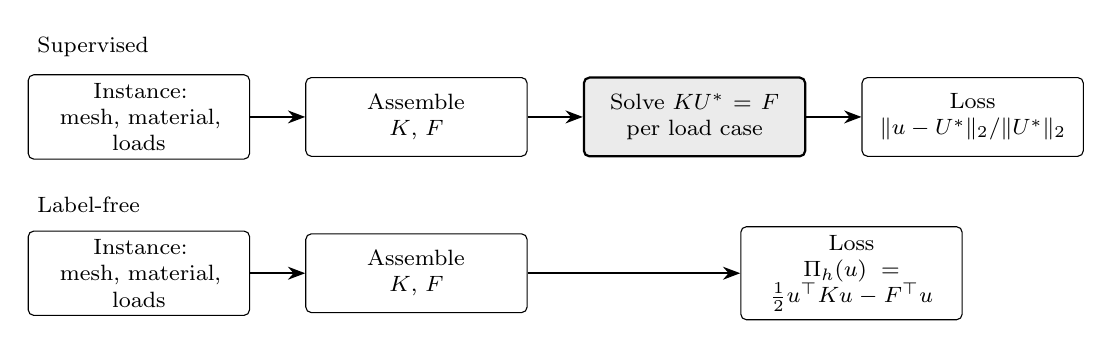
\begin{tikzpicture}[
  node distance=5mm and 7mm,
  box/.style={draw, rounded corners=2pt, align=center, font=\footnotesize,
              minimum height=10mm, text width=26mm, inner sep=3pt},
  cost/.style={box, fill=black!8, thick},
  arr/.style={-{Stealth[length=2.2mm]}, semithick}]
\node[box] (i1) {Instance:\\ mesh, material,\\ loads};
\node[box, right=of i1] (a1) {Assemble\\ $K$, $F$};
\node[cost, right=of a1] (s1) {Solve $K\Ustar=F$\\ per load case};
\node[box, right=of s1] (l1) {Loss\\ $\norm{u-\Ustar}_2/\norm{\Ustar}_2$};
\node[box, below=9mm of i1] (i2) {Instance:\\ mesh, material,\\ loads};
\node[box, right=of i2] (a2) {Assemble\\ $K$, $F$};
\node[box, right=27mm of a2] (l2) {Loss\\ $\Pi_h(u)=\tfrac12u^{\top}Ku-F^{\top}u$};
\draw[arr] (i1) -- (a1);
\draw[arr] (a1) -- (s1);
\draw[arr] (s1) -- (l1);
\draw[arr] (i2) -- (a2);
\draw[arr] (a2) -- (l2);
\node[font=\footnotesize, anchor=south west] at ([yshift=1mm]i1.north west) {Supervised};
\node[font=\footnotesize, anchor=south west] at ([yshift=1mm]i2.north west) {Label-free};
\end{tikzpicture}
\caption{The two training routes for the same network. Supervised training needs a
reference solution for every training instance and load case (shaded); label-free
training evaluates the assembled discrete potential energy of the prediction $u$, which by
\cref{lem:exact} differs from the stiffness-norm regression loss by a constant.}
\label{fig:schematic}
\end{figure}

\Cref{fig:schematic} contrasts the two routes. The label-free transformer minimises
\eqref{eq:training} with $L=4$: at each step one training instance is drawn, without
replacement within an epoch, its four load cases are predicted, and the mean of their
energies is the loss; no reference solution is read. The supervised transformer, the same
network, minimises on labelled instances the mean over the load cases of the relative
displacement error,
\begin{equation}
\mathcal{L}_D=\frac{1}{L}\sum_{j=1}^{L}\frac{\norm{u_j-\Ustar_j}_2}{\norm{\Ustar_j}_2},
\label{eq:ld}
\end{equation}
where $u_j$ is the prediction and $\Ustar_j$ the reference solution for load case $j$ of an
instance, and $F_j$ its load vector. In two dimensions the same network was also trained on
the relative stiffness-norm error,
\begin{equation}
\mathcal{L}_K=\frac{1}{L}\sum_{j=1}^{L}\frac{\norm{u_j-\Ustar_j}_K}{\norm{\Ustar_j}_K}
=\frac{1}{L}\sum_{j=1}^{L}g(u_j)^{1/2},
\label{eq:lk}
\end{equation}
which replaces the norm of \eqref{eq:ld} and nothing else; we call this network the
stiffness-norm transformer. Since
$\norm{u_j-\Ustar_j}_K^2=u_j^{\top}Ku_j-2F_j^{\top}u_j+F_j^{\top}\Ustar_j$, the loss
$\mathcal{L}_K$ uses each reference solution only through the number
$\norm{\Ustar_j}_K^2=F_j^{\top}\Ustar_j$, and its gradient with respect to $u_j$,
\begin{equation}
\nabla_{u_j}\mathcal{L}_K=\frac{Ku_j-F_j}{L\,\norm{u_j-\Ustar_j}_K\,\norm{\Ustar_j}_K},
\label{eq:lkgrad}
\end{equation}
is that of the label-free objective of one instance, $(Ku_j-F_j)/L$, weighted per load case.
The supervised transformer with an energy term adds the mean energy of the four load cases
to $\mathcal{L}_D$, with the gradient of the energy scaled to at most the norm of the
gradient of $\mathcal{L}_D$: the update direction is
$\nabla_\theta\mathcal{L}_D+\min\{1,\norm{\nabla_\theta\mathcal{L}_D}/\norm{\nabla_\theta\bar\Pi}\}\nabla_\theta\bar\Pi$,
with $\bar\Pi$ the mean energy. In three dimensions with 16 labelled instances the energy
term was instead $\bar\Pi$ divided by the mean of $\lvert\Pi_h(\Ustar)\rvert$ over the load
cases, with weight one, a policy fixed in the three-dimensional pre-registration after an
exploratory two-dimensional run had shown the scaled form to scatter widely across seeds
with 16 labels (\ref{app:prereg}). The two-dimensional run of July 2026 also trained the
supervised objective from the label-free network's parameters. The graph network is trained
on $\mathcal{L}_D$.

All networks were trained with AdamW \cite{Loshchilov2019} (weight decay $10^{-4}$,
gradient norm clipped at 1) for 200 epochs, with a cosine learning-rate schedule after a
linear warm-up over the first 5\% of the steps, at a peak learning rate of $10^{-3}$
(label-free) or $1.5\times10^{-3}$ (supervised), in single precision with TF32 matrix
products (TensorFloat-32: the inputs of each product rounded to a 10-bit mantissa, the
products accumulated in single precision), each with three seeds (0, 1, 2). The learning rates were fixed before the runs
and not tuned on them; the stiffness-norm transformer used the supervised settings
unchanged. The supervised networks were trained with 16, 64, 256 and 1,024 labelled
instances, the first 16, 64, 256 and 1,024 instances of the training pool. The label-free
network was trained on the same 1,024 instances without their solutions, for 204,800 steps;
its training set is thus the supervised networks' largest one with the labels removed. In
the two-dimensional comparison of \cref{sec:results2d}, the label-free networks are those
trained in the run of 29 September 2026 (\ref{app:e1}) with these settings and the later
code, evaluated without retraining; at a given seed the transformers start from the same
initial weights and, with 1,024 instances, see them in the same sequence of per-epoch
permutations, so that the supervised and the stiffness-norm transformers differ only in the
loss. Except in
the two-dimensional run of July 2026, the graph network was trained with 64 and 1,024
labelled instances only, a saving of machine time fixed in the pre-registrations. The
networks of the secondary checks of \cref{sec:results2d:decisions,sec:results2d:other} were
trained with the settings given where they are reported.

\subsection{Metrics}\label{sec:methods:metrics}

For each validation instance and load case we compute five metrics. The relative
displacement error is $\norm{u-\Ustar}_2/\norm{\Ustar}_2$. The relative energy gap is
$g(u)$ of \eqref{eq:relgap}, computed as $\gap(u)/\lvert\Pi_h(\Ustar)\rvert$. With the
element-wise von Mises stresses $\vm(u)$ and $\vm(\Ustar)$, which are constant on linear
elements, the von Mises error is
$\norm{\vm(u)-\vm(\Ustar)}_2/\norm{\vm(\Ustar)}_2$, the norms taken over the vector of
element values; the peak stress error is
$\lvert\max\vm(u)-\max\vm(\Ustar)\rvert/\max\vm(\Ustar)$; and the critical-region recall is
the share of the $n_c$ elements with the largest $\vm(\Ustar)$ that are also among the
$n_c$ elements with the largest $\vm(u)$, with $n_c$ the nearest integer to a tenth of the
number of elements. Each metric is averaged over the four load cases of an instance and
then over the 256 validation instances; tables give the mean and the sample standard
deviation over the three seeds. The relative energy gap is the primary metric, as
pre-registered: by \cref{prop:stress} it is the strain energy of the stress error relative
to that of the solution, and by \cref{cor:zero} a prediction with $g>1$ is worse than the
zero field.

\subsection{Pre-registration}\label{sec:methods:prereg}

Each run whose results decide a claim of this paper was specified, before it was executed,
in a pre-registration document that fixes the configuration, the metrics, the decision
gates and the kill conditions, which withdraw a claim when they are triggered; both
outcomes of every such run were declared publishable in advance. The configuration is
identified by its SHA-256 hash, and the code refused to start a run whose configuration did
not match the registered hash. Each run was carried out once. The documents of the
three-dimensional runs, of the runs of \ref{app:e1} and \cref{sec:cost:training} and of
the two-dimensional comparison of \cref{sec:results2d} were committed and pushed to the
project's public repository before their runs; tags mark the commits. Those of the
two-dimensional runs of July 2026 carried their configuration hashes, which the code checked
at start-up, but were committed to the repository only on 3 August 2026, after the runs;
their content at the time of the runs rests on the authors' archives, whose hashes the
repository's provenance note records (\ref{app:prereg}). The initial
three-dimensional run needed eight attempts because of memory and process faults; each
restart reused the networks already trained under the same registered configuration, and
the engineering changes the restarts needed are recorded as leaving every value unchanged.
Results that were not pre-registered, an exploratory replication (\cref{sec:results2d:other})
and readings taken after the runs (\cref{sec:results2d:spectrum,sec:results3d:reverse,%
sec:results3d:detection,sec:transfer:amplitude}), are labelled as such.
\Cref{tab:criteria} in \ref{app:prereg} lists every pre-registered criterion of these runs
with its outcome, met or not, under the labels of the pre-registration documents, which
the table explains. An independent script recomputed the three-dimensional verdict from the
report.

Four departures from the plans bear on the reading of the results and are described in
\ref{app:prereg}. First, the initial three-dimensional run (21 September 2026) used a
label-free objective that omitted the output scaling by $F_{\max}$, which inference applied,
so that the trained label-free network returned about \numDfourteenAlpha{} times the
solution (deviation D14). A pre-registered amendment repeated only what depended on that
objective, with the corrected code, and reused the supervised networks, which it had not affected, after
checking their hashes; \cref{sec:results3d,sec:transfer} report the amended run of
28 September 2026. Second, the same amendment, decided after the results of the initial run
were known, assessed one sanity condition only at label budgets of 64 and above; we report
the gate under both readings. Third, the three-dimensional pre-registration text stated
that the label-free network would train on 1,744 instances, whereas the registered
configuration, which is what ran, trained it on the same 1,024 instances as the supervised
networks (deviation D16); the comparison is therefore the one described above. Fourth, a
pre-registered two-dimensional comparison of 31 July 2026 kept, under its decision rule, a
self-supervised term in the pretraining objective; this paper reports the energy objective
without it, a scope chosen after that result was known.

\paragraph{Field plots}
The instances shown in the field plots of \cref{sec:results2d,sec:results3d,sec:transfer}
were chosen by rules fixed in code before any field was drawn: in two dimensions, the
validation instance with the median relative energy gap of the supervised transformer; in
three dimensions, the validation instance with the largest relative energy gap of the
supervised transformer (the same instance in all three seeds), the validation instance with
the median relative energy gap of the label-free transformer, and the fine-mesh instance
with the median displacement error of the label-free transformer; each in seed 0, the median
of $n$ values being the lower one, of rank $\lfloor(n-1)/2\rfloor$ counted from zero in
ascending order. The first three-dimensional rule, and the two-dimensional rule, which was
written after the verdict of the run of 9 October 2026, were chosen after the per-instance
records had been examined, but before any field had been plotted. Each plot shows one load case of its instance, chosen by
the same rule applied to the instance's four load cases (the largest value, or the second
smallest); this was fixed when the plots were made, after the per-load-case values had been
examined but before any field had been drawn. The three-dimensional plots show the three
faces of the box seen in an oblique projection, the free end on the right; the clamped face
and the cavities are hidden.

\section{Results in two dimensions}\label{sec:results2d}

The two-dimensional comparison is the pre-registered run of 9 October 2026, made with the
later code of \cref{sec:methods:networks}, which multiplies the decoded field by $F_{\max}$
as in three dimensions. It trained again two networks of an earlier pre-registered run,
that of 16 July 2026, on the same corpus, split and seeds and with the same training
settings: the supervised transformer, with every number of labelled instances, and the
graph network, with 64 and 1,024 only (\cref{sec:methods:training}). Beside them it
evaluated, without retraining them, the three label-free transformers that the run of 29
September 2026 had trained with the same code on the same 1,024 instances (the
unregularised networks of \ref{app:e1}). It added one network, the stiffness-norm
transformer: the supervised transformer trained on the relative stiffness-norm error
\eqref{eq:lk} instead of the relative displacement error \eqref{eq:ld}, with the same
labels, which separates the norm of the loss from the labels (\cref{sec:results2d:norm}).
The trained networks of this section are thus the label-free, the supervised and the
stiffness-norm transformers and the graph network. The run of 16 July 2026 is reported in
\cref{sec:results2d:july}; the configuration hashes of both runs are given in
\ref{app:repro}.

\subsection{Accuracy}\label{sec:results2d:accuracy}

% generated by scripts/make_cmame_material.py from the records; do not edit
\begin{table}[tbp]
\centering
\footnotesize
\setlength{\tabcolsep}{4pt}
\caption{Two-dimensional plates, every metric at the largest label budget. The supervised networks were trained on 1,024 labelled instances; the label-free network on the same 1,024 instances without their solutions.}
\label{tab:2d}
\resizebox{\ifdim\width>\textwidth\textwidth\else\width\fi}{!}{%
\begin{tabular}{lcccccc}
\toprule
Model & \shortstack{Displacement \\ error} & \shortstack{Relative \\ energy gap} & \shortstack{von Mises \\ error} & \shortstack{Peak stress \\ error} & \shortstack{Critical-region \\ recall} & \shortstack{Worse than \\ zero field} \\
\midrule
Label-free & 0.166 $\pm$ 0.002 & 0.0817 $\pm$ 0.0040 & 0.210 $\pm$ 0.003 & 0.228 $\pm$ 0.001 & 0.739 $\pm$ 0.003 & 3/768 \\
Supervised & 0.160 $\pm$ 0.003 & 0.418 $\pm$ 0.037 & 0.433 $\pm$ 0.031 & 0.334 $\pm$ 0.036 & 0.584 $\pm$ 0.027 & 52/768 \\
Supervised + energy term & 0.161 $\pm$ 0.005 & 0.166 $\pm$ 0.040 & 0.257 $\pm$ 0.007 & 0.246 $\pm$ 0.022 & 0.708 $\pm$ 0.012 & 14/768 \\
Label-free, then supervised & 0.166 $\pm$ 0.006 & 0.236 $\pm$ 0.032 & 0.336 $\pm$ 0.020 & 0.301 $\pm$ 0.019 & 0.645 $\pm$ 0.008 & 21/768 \\
Graph network, supervised & 0.167 $\pm$ 0.000 & 2.57 $\pm$ 0.25 & 1.10 $\pm$ 0.07 & 1.32 $\pm$ 0.13 & 0.322 $\pm$ 0.027 & 481/768 \\
\midrule
Nearest-neighbour field & 0.404 & 0.959 & 0.735 & 0.643 & 0.515 & 94/256 \\
Scaled polynomial & 1.42 & 873 & 11.4 & 30.8 & 0.159 & 256/256 \\
\midrule
Zero field & 1.00 & 1.00 & 1.00 & 1.00 & -- & -- \\
\bottomrule
\end{tabular}}

\smallskip
\begin{minipage}{\linewidth}\footnotesize\raggedright
256 validation instances, never trained on; four load cases each. Errors are relative to the reference finite-element solution, per load case, then averaged over the load cases; the relative energy gap of the zero field is 1. Trained networks: mean $\pm$ sample standard deviation over 3 seeds; the nearest-neighbour field and the scaled polynomial are deterministic.\par
Worse than zero field: instance-seed pairs whose relative energy gap exceeds 1, that is, predictions further from the solution in the energy norm than the zero field.\par
Critical-region recall: the share of the 10\% most stressed elements of the reference solution that are also among the 10\% most stressed of the prediction (higher is better; in every other column lower is better).\par
Run of 16 July 2026. Its code did not multiply the load scale back onto the output (\cref{sec:methods:networks}); we attribute the narrow spread of the displacement errors to this, untested (\cref{sec:results2d:other}).
\end{minipage}
\end{table}


\Cref{tab:2d} gives every metric with 1,024 labelled instances. The label-free transformer
was more accurate than the supervised transformer, the same network trained on the solutions
of the same instances, on every metric but the displacement error, in each of the three
seeds: its relative energy gap, \numCmFreeGap{}, was \numCmLabOverFreeGap{} times lower, and
its von Mises error (\numCmFreeVm{} against \numCmLabVm{}), peak stress error
(\numCmFreePeak{} against \numCmLabPeak{}) and critical-region recall (\numCmFreeRecall{}
against \numCmLabRecall{}) were better. Its displacement error, \numCmFreeDispFour{}, was
\numCmFreeDispExcessAbs{} higher than the supervised transformer's, \numCmLabDispFour{}, and
higher in each seed, by \numCmFreeDispExcessMin{} to \numCmFreeDispExcessMax{}. Compared
instance by instance within each seed, the label-free transformer had the lower relative
energy gap on \numPairCmLabGap{} of the \numCmPairs{} instance-seed pairs and the lower von
Mises error on \numPairCmLabVm{}, but the lower displacement error on only
\numPairCmLabDisp{}; on \numPairCmOpposite{} of the pairs the displacement error and the von
Mises error ranked the two networks in opposite orders (\cref{rem:rank}).

The pre-registered hypothesis H1, that the label-free transformer has the lower relative
energy gap, was supported: its seed mean was \numHOneRel{} lower, beyond the noise guard of
\numHOneTau{}. The guard, fixed in the pre-registration, is the larger of 10\% and twice the
standard error of the relative difference of the two seed means (note to
\cref{tab:criteria}); a difference within it is reported as no difference shown, which is
not equivalence. \Cref{tab:cm2d} gives, for H1 and the other hypotheses of this run, the
per-seed values and the readings that the pre-registration required beside each verdict:
on the seeds' medians over the instances the guard gave the same readings, and the 95\%
intervals of the relative difference, from Welch's statistic over the seeds and from
resampling the instances, lay below zero for H1, H2a and H2b.

As in three dimensions (\cref{sec:results3d:reverse}), the graph network had the lowest
displacement error in the table, \numCmMgnDisp{}, \numCmMgnBelowLabDisp{} below the
supervised transformer's and within the noise guard of it, and stress errors several times
the label-free transformer's: its von Mises error was \numCmMgnOverFreeVm{} times the
label-free transformer's, and its relative energy gap, \numCmMgnGap{} against
\numCmFreeGap{}, was the largest of the trained networks, \numCmMgnOverLabGap{} times even the
supervised transformer's. Against the supervised transformer, instance by instance, it had
the lower displacement error on \numPairCmMgnLabDisp{} of the pairs, the lower relative
energy gap on \numPairCmMgnLabGap{} and the lower von Mises error on \numPairCmMgnLabVm{}.
Of its \numCmPairs{} instance-seed predictions, \numCmMgnWorse{} were further from the
solution, in the energy norm, than the zero field, against none for each of the three
transformers. Taken load case by load case after the run, over the \numSpecLoads{} triples
of seed, instance and load case of \cref{sec:results2d:spectrum}, \numSpecLoadWorseMgn{} of
the graph network's predictions were worse than the zero field, against
\numSpecLoadWorseFree{} for the label-free transformer, \numSpecLoadWorseLab{} for the
supervised transformer and \numSpecLoadWorseKnorm{} for the stiffness-norm transformer.

\subsection{Supervision in the stiffness norm}\label{sec:results2d:norm}

The supervised and the label-free transformers differ chiefly in the labels and in the norm
of the loss, the Euclidean norm of \eqref{eq:ld} against the stiffness norm in which, by
\cref{cor:training}, the energy regresses; they also weight the load cases differently and
were trained at different learning rates (\cref{sec:methods:training}). The stiffness-norm
transformer keeps the labels and changes the norm. At a given seed it starts from the same
initial weights as the supervised transformer and visits the instances in the same
sequence, so the two differ only in the loss (\cref{sec:methods:training}). Two hypotheses
about it were pre-registered: H2a, that its relative energy gap is lower than the
supervised transformer's, which is close to a check that the change of loss took effect,
since \eqref{eq:lk} averages the square roots of the relative energy gaps; and H2b, that its
von Mises error is lower. The von Mises error is a term of neither loss, and by
\cref{prop:stress} the stiffness-norm error is the compliance-weighted stress error and
bounds the area-weighted von Mises error: H2b tests the explanation this paper gives for the
label-free network's accurate stresses (\cref{sec:discussion}).

Both were supported. With 1,024 labelled instances the stiffness-norm transformer's relative
energy gap was \numHTwoARel{} lower than the supervised transformer's (guard
\numHTwoATau{}), and its von Mises error \numHTwoBRel{} lower, \numCmKnormVm{} against
\numCmLabVm{} (guard \numHTwoBTau{}). It had the lower relative energy gap on
\numPairCmKnormLabGap{} of the instance-seed pairs, the lower von Mises error on
\numPairCmKnormLabVm{} and the lower displacement error on \numPairCmKnormLabDisp{}: changing
the norm halved the von Mises error and left the displacement error about where it was,
\numCmKnormDisp{} against \numCmLabDisp{}. Weighted by element area, as in
\cref{prop:stress}, instead of equally, the ratio of the two networks' mean von Mises errors
was \numSpecVmAreaRatio{}, against \numSpecVmElemRatio{} for the reported metric (measured
after the run, \cref{sec:results2d:spectrum}).

A third comparison, H3, was pre-registered as a reading without a criterion: the
stiffness-norm transformer against the label-free transformer. It showed no difference
beyond the guard, which is not equivalence. The stiffness-norm transformer's relative energy
gap, \numCmKnormGap{}, was \numHThreeRel{} lower, within the guard of \numHThreeTau{}, which
its seeds made wide (\numCmKnormGapSeeds{}, against \numCmFreeGapSeeds{}); with the
stiffness-norm transformer as the reference instead, the label-free transformer's was
\numHThreeExRel{} higher, within the guard of \numHThreeExTau{}. In every seed the
stiffness-norm transformer was the more accurate of the two on every metric, by
\numHThreeSeedRel{} in relative energy gap in seeds 0, 1 and 2: seed 1 makes most of the
difference between the seed means (seeds 0 and 2 alone give \numHThreeSeedsZeroTwo{}) and,
through the spread it adds, most of the width of the guard. Instance by instance, the
stiffness-norm transformer had the lower relative energy gap on \numPairCmKnormFreeGap{} of
the pairs, the lower von Mises error on \numPairCmKnormFreeVm{} and the lower displacement
error on \numPairCmKnormFreeDisp{}, and resampling the instances, with the seeds kept, put
its relative energy gap \numHThreeResLow{} to \numHThreeResHigh{} below the label-free
transformer's (95\% interval, \cref{tab:cm2d}); the guard, which treats the three seeds as
the replicates, does not separate the two networks. H3 compares two networks rather than
training with and without labels: by \eqref{eq:lkgrad} the two objectives weight the same
residual differently per load case, and the two networks were trained at different learning
rates.

\subsection{Where the errors lie in the spectrum}\label{sec:results2d:spectrum}

\Cref{rem:factor} writes the relative energy gap of a prediction as the product of the
squared relative displacement error $\delta^2$ and the normalised Rayleigh quotient $\rho$,
which measures how far up the spectrum of $K$ the error lies relative to the solution. After
the run, and without pre-registration, we measured both for the four trained networks with
1,024 labelled instances on each of the \numSpecLoads{} triples of seed, validation instance
and load case, and, from the eigendecomposition of each instance's stiffness matrix
(\numSpecFreeMin{} to \numSpecFreeMax{} free degrees of freedom), how each error's squared
stiffness norm is distributed over the eigenmodes. The solution itself lies at the bottom of
the spectrum: its Rayleigh quotient was a median \numSpecRqStarOverMin{} times the smallest
eigenvalue of $K$. The errors lay higher (\cref{fig:spectra}): the median of $\rho$ was
\numSpecRqFree{} for the label-free transformer, \numSpecRqKnorm{} for the stiffness-norm
transformer, \numSpecRqLab{} for the supervised transformer and \numSpecRqMgn{} for the
graph network.

\begin{figure}[tbp]
\centering
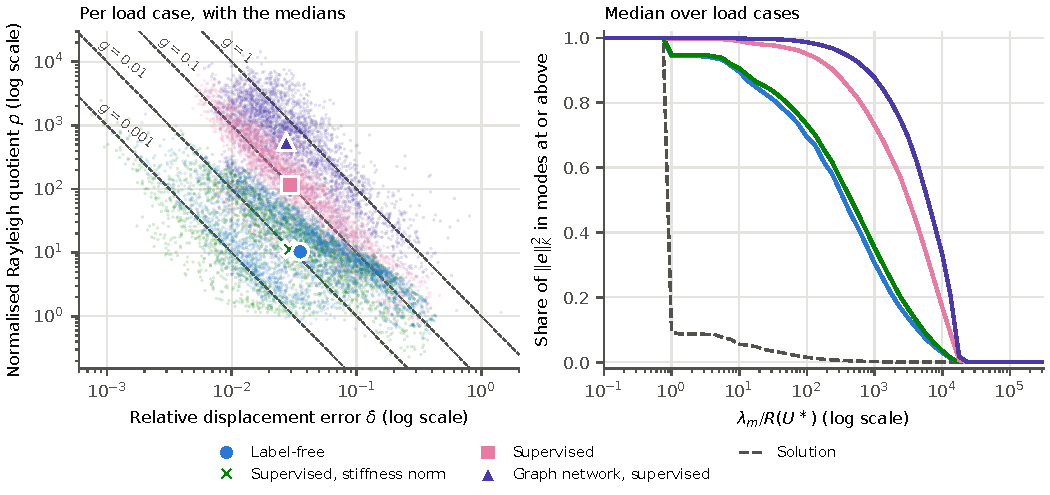
\includegraphics[width=\linewidth]{generated/fig_spectra.pdf}
\caption{Two dimensions, 1,024 labelled instances, measured after the run: where the errors
lie in the spectrum of the stiffness matrix. Left: for each of the \numSpecLoads{} triples
of seed, validation instance and load case (one point per triple and network), the
normalised Rayleigh quotient $\rho$ of the error against the relative displacement error
$\delta$ (\cref{rem:factor}); large markers are the medians of the two coordinates, and the
dashed lines are lines of equal relative energy gap $g=\rho\,\delta^2$. Right: for each
value of $\lambda_m/R(\Ustar)$ on the abscissa, the median over the triples of the share of
the error's squared stiffness norm in the eigenmodes at or above it; the dashed curve is the
same share of the solution's squared stiffness norm.}
\label{fig:spectra}
\end{figure}

The supervised and the stiffness-norm transformers, which differ only in the norm of the
loss, had errors of about the same size in different places. Over the triples, the geometric
mean of the ratio of their $\rho$, supervised over stiffness-norm, was \numSpecLabKnormRq{}
(\numSpecLabKnormRqSeeds{} in seeds 0, 1 and 2), and the supervised transformer's $\rho$ was
the larger on \numSpecLabKnormAbove{} of the triples. When each network's $\rho$ is first
averaged geometrically over its three seeds, which does not pair the seeds of the two
networks, the supervised transformer's was the larger on \numSpecLabKnormAboveSeedGm{} of
the \numSpecLoadCases{} pairs of instance and load case. The geometric mean of the ratio of
their $\delta^2$ was \numSpecLabKnormDisp{} (\numSpecLabKnormDispSeeds{}), and the
supervised transformer's $\delta$ was the smaller on \numSpecLabKnormDispLower{} of the
triples.

By \eqref{eq:factor}, the geometric mean of the ratio of their relative energy gaps,
\numSpecLabKnormGap{}, is the product of the two. On a logarithmic scale the ratio of $\rho$
accounts for \numSpecSpectralShare{} of it and the ratio of $\delta^2$ for the rest
(\numSpecSpectralShareMin{} to \numSpecSpectralShareMax{} in the three seeds; in the seed in
which the supervised transformer's errors were the smaller, the ratio of $\rho$ accounts for
more than the whole). This geometric mean is not the ratio of the seed means that H2a
tested, \numCmLabOverKnormGap{}, which the largest errors dominate. The modes with
$\lambda_m\ge 100\,R(\Ustar)$ held a median \numSpecShareKLab{} of the squared stiffness norm
of the supervised transformer's error, against \numSpecShareKKnorm{} for the stiffness-norm
transformer, \numSpecShareKFree{} for the label-free transformer and \numSpecShareKStar{} of
the solution's own.

The graph network's errors had the size of the supervised transformer's (ratio of
$\delta^2$, graph network over supervised, \numSpecMgnLabDisp{}) and lay higher still (ratio
of $\rho$ \numSpecMgnLabRq{}). The stiffness-norm and the label-free transformers, trained in
the same norm, had errors at the same place in the spectrum (ratio of $\rho$, stiffness-norm
over label-free, \numSpecKnormFreeRq{}) and of different sizes (ratio of $\delta^2$
\numSpecKnormFreeDisp{}; \numSpecKnormFreeDispSeeds{} in the three seeds): the
stiffness-norm transformer's errors were the smaller in every seed, by far the smaller in
seed 1, the seed that makes most of the difference in H3 (\cref{sec:results2d:norm}).

\begin{figure}[tbp]
\centering
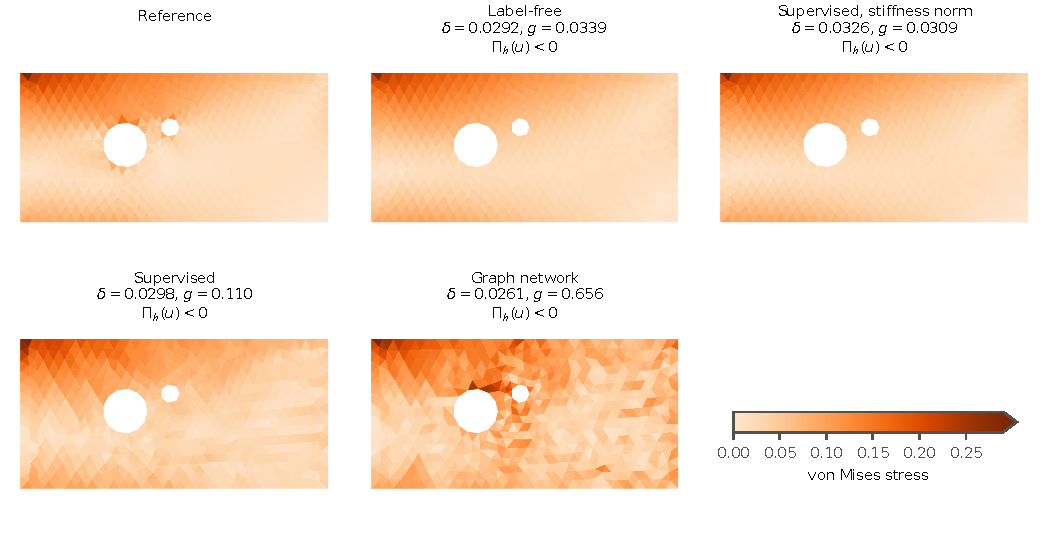
\includegraphics[width=\linewidth]{generated/fig_field2d.pdf}
\caption{Two dimensions, validation instance No.~\numSpecFigIndex{}, the one with the median
relative energy gap of the supervised transformer, seed 0, under the \numFigTwoDLoad{}
(selection rules in \cref{sec:methods:prereg}). Von Mises stress of the reference solution
and of the four networks with 1,024 labelled instances, on one colour scale set by the
reference. First row: the reference, then the two networks trained in the stiffness norm
(the label-free and the stiffness-norm transformers); second row: the two trained on the
displacement error (the supervised transformer and the graph network). Above each network,
its relative displacement error $\delta$ and relative energy gap $g$ on this load case and
the sign of $\Pi_h(u)$.}
\label{fig:field2d}
\end{figure}

\Cref{fig:field2d} shows one instance, chosen by the rule of \cref{sec:methods:prereg}
before the run's spectra were exported, in the load case that the same rule picks among its
four. On that load case, the four networks' displacement errors lay between
\numFigTwoDDispMin{} and \numFigTwoDDispMax{} and their relative energy gaps between
\numFigTwoDGapMin{} and \numFigTwoDGapMax{}; the stress fields of the two networks trained on
the displacement error are visibly rougher.

The networks ran with TF32 matrix products (\cref{sec:methods:training}), whose rounding
varies from node to node and therefore weighs heavily in the energy norm, so each network was
also evaluated with TF32 off. The rounding, the difference between the two predictions, had
a squared stiffness norm of a median \numSpecTfFree{} and \numSpecTfKnorm{} of that of the
error for the label-free and the stiffness-norm transformers (\numSpecTfLab{} and
\numSpecTfMgn{} for the two networks trained on the displacement error). In the modes with
$\lambda_m\ge10^4R(\Ustar)$ it had a median \numSpecTfStiffFree{} and
\numSpecTfStiffKnorm{} of the error's squared stiffness norm in those modes, on the
\numSpecTfStiffN{} triples whose spectra reach that far (\numSpecTfStiffLoads{} of the
\numSpecLoadCases{} pairs of instance and load case, in each seed). With TF32 off, the
median quotients $\rho$ were \numSpecIeeeRqFree{} (label-free), \numSpecIeeeRqKnorm{}
(stiffness norm), \numSpecIeeeRqLab{} (supervised) and \numSpecIeeeRqMgn{} (graph network),
and the geometric-mean ratios of $\rho$ and of $g$ between the supervised and the
stiffness-norm transformers rose to \numSpecIeeeLabKnormRq{} and \numSpecIeeeLabKnormGap{}.
The rounding thus places the errors of the two networks trained in the stiffness norm higher
in the spectrum than they would lie without it, and the readings as run understate the
differences between the networks trained in the two norms.

\subsection{Label efficiency}\label{sec:results2d:labels}

% generated by scripts/make_cmame_material.py from the records; do not edit
\begin{table}[tbp]
\centering
\footnotesize
\setlength{\tabcolsep}{4pt}
\caption{Label efficiency: relative displacement error / relative energy gap against the number of labelled training instances (seed means).}
\label{tab:labeleff}
\resizebox{\ifdim\width>\textwidth\textwidth\else\width\fi}{!}{%
\begin{tabular}{llcccc}
\toprule
Run & Model & 16 & 64 & 256 & 1,024 \\
\midrule
2D & Supervised & 0.459 / 20.8 & 0.165 / 3.06 & 0.0712 / 0.430 & 0.0505 / 0.133 \\
2D & Supervised, stiffness norm & 0.362 / 0.254 & 0.0889 / 0.0505 & 0.0667 / 0.0383 & 0.0547 / 0.0290 \\
2D & Graph network, supervised & -- & 0.370 / 149 & -- & 0.0499 / 0.825 \\
2D & Nearest-neighbour field & 0.687 / 6.50 & 0.466 / 1.65 & 0.408 / 1.03 & 0.404 / 0.959 \\
2D & Label-free (no labels) & 0.0634 / 0.0383 & 0.0634 / 0.0383 & 0.0634 / 0.0383 & 0.0634 / 0.0383 \\
\midrule
2D, July & Supervised & 0.272 / 6.26 & 0.193 / 2.72 & 0.176 / 1.26 & 0.160 / 0.418 \\
2D, July & Supervised + energy term & 0.410 / 2.56 & 0.184 / 0.579 & 0.182 / 0.154 & 0.161 / 0.166 \\
2D, July & Label-free, then supervised & 0.207 / 1.32 & 0.189 / 0.201 & 0.181 / 0.302 & 0.166 / 0.236 \\
2D, July & Graph network, supervised & 0.684 / 92.6 & 0.425 / 80.6 & 0.181 / 7.55 & 0.167 / 2.57 \\
2D, July & Label-free (no labels) & 0.166 / 0.0817 & 0.166 / 0.0817 & 0.166 / 0.0817 & 0.166 / 0.0817 \\
\midrule
3D & Supervised & 0.395 / 18.5 & 0.288 / 5.95 & 0.0726 / 0.799 & 0.0470 / 31.2 \\
3D & Supervised + energy term & 0.369 / 0.621 & 0.256 / 0.854 & 0.0833 / 0.964 & 0.0470 / 0.116 \\
3D & Graph network, supervised & -- & 0.149 / 18.3 & -- & 0.0168 / 0.447 \\
3D & Nearest-neighbour field & 0.648 / 5.74 & 0.477 / 2.24 & 0.400 / 1.20 & 0.382 / 1.22 \\
3D & Label-free (no labels) & 0.0300 / 0.00912 & 0.0300 / 0.00912 & 0.0300 / 0.00912 & 0.0300 / 0.00912 \\
\bottomrule
\end{tabular}}

\smallskip
\begin{minipage}{\linewidth}\footnotesize\raggedright
Seed means over 3 seeds (the nearest-neighbour field is deterministic, and the same in both 2D runs). A dash marks a budget at which the model was not trained (the graph network was trained at 64 and 1,024 labels only, except in the 2D run of July 2026). 2D: the run of 9 October 2026 (\cref{tab:2d}); 2D, July: the run of 16 July 2026, with the earlier code (\cref{tab:2djuly}). The label-free row repeats its single value, which uses the same 1,024 instances without labels.
\end{minipage}
\end{table}


\begin{figure}[tbp]
\centering
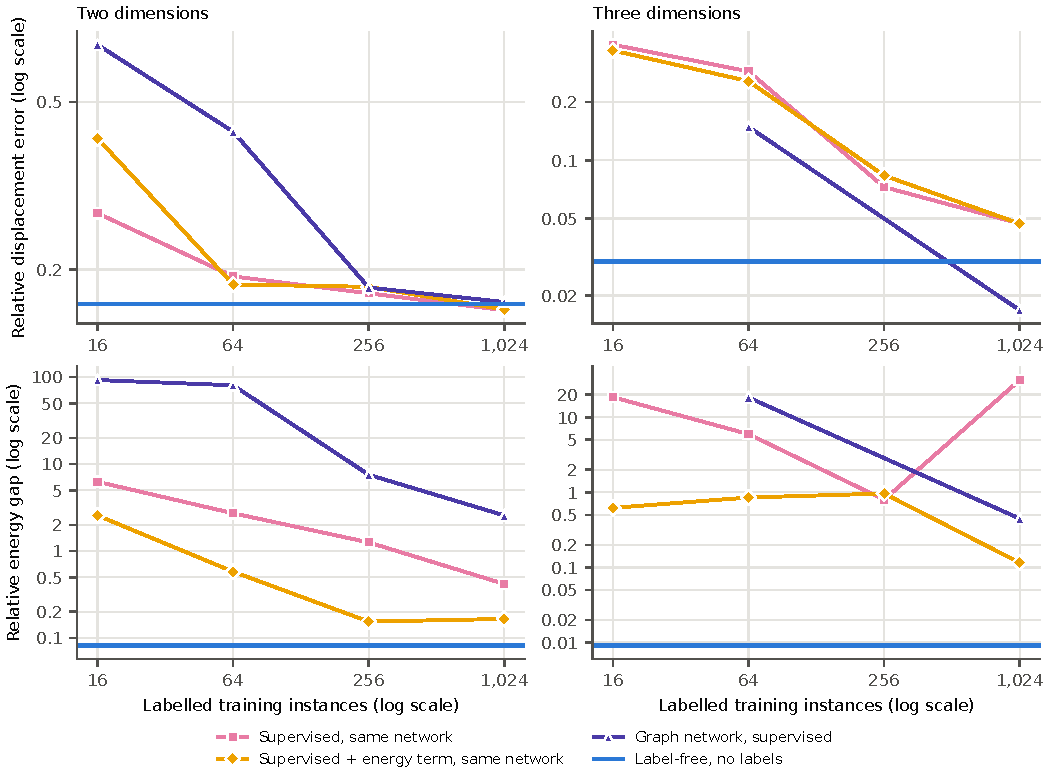
\includegraphics[width=\linewidth]{generated/fig_label_efficiency.pdf}
\caption{Label efficiency in two dimensions (left; the run of 9 October 2026) and three
dimensions (right): seed-mean relative displacement error (top) and relative energy gap
(bottom) of the supervised networks against the number of labelled training instances. The
horizontal line is the label-free transformer, trained on the same 1,024 instances without
their solutions. The stiffness-norm transformer was trained in two dimensions only, and the
graph network, in both panels, with 64 and 1,024 labels only; the supervised transformer
with the energy term is shown in three dimensions only (its two-dimensional values, from
the run of 16 July 2026, are in \cref{tab:labeleff}).}
\label{fig:labeleff}
\end{figure}

\Cref{tab:labeleff} and \cref{fig:labeleff} give the errors of the supervised networks
against the number of labelled instances. With no labels, the label-free transformer's
relative energy gap was lower than the supervised transformer's and the graph network's at
every budget; its advantage over the supervised transformer,
$1-g_{\text{label-free}}/g_{\text{supervised}}$ for the seed means, fell from
\numCmAdvMax{} with 16 labels to \numCmAdvMin{} with 1,024. In displacement, the supervised
transformer and the graph network needed 1,024 labels to pass it.

The pre-registration also compared the supervised and the stiffness-norm transformers with
the label-free transformer on every metric at every budget, by the same guard, as readings
without verdicts. These are among its \numCmSecondary{} secondary readings, which are
exploratory and not corrected for multiplicity, so that some crossings of the guard are
expected by chance. The supervised transformer was worse than the label-free transformer
beyond the guard in relative energy gap, von Mises error, peak stress error and
critical-region recall at every budget. The stiffness-norm transformer was worse beyond the
guard on every metric with 16 labelled instances and on every metric but the
critical-region recall with 64, and within the guard on every metric with 256 and 1,024;
its seed means fell below the label-free transformer's, in relative energy gap and in
displacement, with 1,024 labels only. With 16, 64 and 256 labelled instances,
\numCmLabWorseSixteen{}, \numCmLabWorseSixtyFour{} and \numCmLabWorseTwoFiveSix{} of the
supervised transformer's \numCmPairs{} instance-seed predictions were worse than the zero
field, against \numCmKnormWorseSixteen{}, \numCmKnormWorseSixtyFour{} and
\numCmKnormWorseTwoFiveSix{} for the stiffness-norm transformer. Supervised in the stiffness
norm, 256 labelled instances brought the transformer's seed means within the guard of the
label-free transformer's on every metric, although the label-free transformer still had the
lower relative energy gap on \numPairCmFreeKnormGapTwoFiveSix{} of the instance-seed pairs;
supervised on the displacement error, 1,024 left a von Mises error \numCmLabOverFreeVm{}
times the label-free transformer's.

\subsection{The run of 16 July 2026}\label{sec:results2d:july}

The run of 16 July 2026, pre-registered before it was executed, compared the networks on the
same corpus, split and seeds with the code of July 2026, in which the decoder did not
multiply $F_{\max}$ back onto the prediction, so that no network in that run could know the
absolute amplitude of an instance's loads (\cref{sec:methods:networks}). It also trained
what the run of 9 October 2026 did not: the supervised transformer with an energy term, the
supervised transformer trained from the label-free transformer's parameters
(\cref{sec:methods:training}), and the graph network with every number of labelled
instances. It trained no stiffness-norm transformer.

\subsubsection{Accuracy and label efficiency}\label{sec:results2d:julyaccuracy}

% generated by scripts/make_cmame_material.py from the records; do not edit
\begin{table}[tbp]
\centering
\footnotesize
\setlength{\tabcolsep}{4pt}
\caption{Two-dimensional plates, the run of 16 July 2026 with the earlier code (\cref{sec:results2d:july}): every metric at the largest label budget, on the instances of \cref{tab:2d}.}
\label{tab:2djuly}
\resizebox{\ifdim\width>\textwidth\textwidth\else\width\fi}{!}{%
\begin{tabular}{lcccccc}
\toprule
Model & \shortstack{Displacement \\ error} & \shortstack{Relative \\ energy gap} & \shortstack{von Mises \\ error} & \shortstack{Peak stress \\ error} & \shortstack{Critical-region \\ recall} & \shortstack{Worse than \\ zero field} \\
\midrule
Label-free & 0.166 $\pm$ 0.002 & 0.0817 $\pm$ 0.0040 & 0.210 $\pm$ 0.003 & 0.228 $\pm$ 0.001 & 0.739 $\pm$ 0.003 & 3/768 \\
Supervised & 0.160 $\pm$ 0.003 & 0.418 $\pm$ 0.037 & 0.433 $\pm$ 0.031 & 0.334 $\pm$ 0.036 & 0.584 $\pm$ 0.027 & 52/768 \\
Supervised + energy term & 0.161 $\pm$ 0.005 & 0.166 $\pm$ 0.040 & 0.257 $\pm$ 0.007 & 0.246 $\pm$ 0.022 & 0.708 $\pm$ 0.012 & 14/768 \\
Label-free, then supervised & 0.166 $\pm$ 0.006 & 0.236 $\pm$ 0.032 & 0.336 $\pm$ 0.020 & 0.301 $\pm$ 0.019 & 0.645 $\pm$ 0.008 & 21/768 \\
Graph network, supervised & 0.167 $\pm$ 0.000 & 2.57 $\pm$ 0.25 & 1.10 $\pm$ 0.07 & 1.32 $\pm$ 0.13 & 0.322 $\pm$ 0.027 & 481/768 \\
\midrule
Nearest-neighbour field & 0.404 & 0.959 & 0.735 & 0.643 & 0.515 & 94/256 \\
Scaled polynomial & 1.42 & 873 & 11.4 & 30.8 & 0.159 & 256/256 \\
\midrule
Zero field & 1.00 & 1.00 & 1.00 & 1.00 & -- & -- \\
\bottomrule
\end{tabular}}

\smallskip
\begin{minipage}{\linewidth}\footnotesize\raggedright
256 validation instances, never trained on; four load cases each. Errors are relative to the reference finite-element solution, per load case, then averaged over the load cases; the relative energy gap of the zero field is 1. Trained networks: mean $\pm$ sample standard deviation over 3 seeds; the nearest-neighbour field and the scaled polynomial are deterministic.\par
Worse than zero field: instance-seed pairs whose relative energy gap exceeds 1, that is, predictions further from the solution in the energy norm than the zero field.\par
Critical-region recall: the share of the 10\% most stressed elements of the reference solution that are also among the 10\% most stressed of the prediction (higher is better; in every other column lower is better).\par
Run of 16 July 2026. Its code did not multiply the load scale back onto the output (\cref{sec:methods:networks}); we attribute the narrow spread of the displacement errors to this; no experiment isolated it (\cref{sec:results2d:julyaccuracy}).
\end{minipage}
\end{table}


\Cref{tab:2djuly} gives every metric with 1,024 labelled instances. The supervised
transformer had the lowest displacement error, \numTwoLabDispFour{} against
\numTwoFreeDispFour{} for the label-free transformer, which was \numTwoFreeDispExcessAbs{}
higher, and higher in each of the three seeds. On every other metric the label-free
transformer was the most accurate network in the table: its relative energy gap,
\numTwoFreeGap{}, was \numTwoLabOverFreeGap{} times lower than the supervised transformer's,
and its von Mises error (\numTwoFreeVm{} against \numTwoLabVm{}), peak stress error
(\numTwoFreePeak{} against \numTwoLabPeak{}) and critical-region recall (\numTwoFreeRecall{}
against \numTwoLabRecall{}) were better. Compared instance by instance within each seed, the
label-free transformer had the lower relative energy gap on \numPairTwoLabGap{} of the
\numTwoPairs{} instance-seed pairs and the lower von Mises error on \numPairTwoLabVm{}, but
the lower displacement error on only \numPairTwoLabDisp{}. The energy term lowered the
supervised transformer's relative energy gap to \numTwoAncGap{} and its von Mises error to
\numTwoAncVm{}, both still above the label-free values. The graph network matched the others
in displacement (\numTwoMgnDisp{}) but had a relative energy gap of \numTwoMgnGap{} and a von
Mises error of \numTwoMgnVm{}: \numTwoMgnWorse{} of its \numTwoPairs{} instance-seed
predictions were further from the solution, in the energy norm, than the zero field. The
supervised transformer had \numTwoLabWorse{} such predictions, the supervised transformer
with the energy term \numTwoAncWorse{}, and the label-free transformer \numTwoFreeWorse{},
one per seed.

The displacement errors of the five trained networks lie between \numTwoLabDisp{} and
\numTwoMgnDisp{}, a narrow band, while their relative energy gaps span a factor of
\numTwoGapSpread{}. We attribute the narrow band to the code: no network could know the
absolute amplitude of an instance's loads, which adds an error common to every displacement
and compresses their differences. With the later code, the displacement errors of the
label-free transformer, the supervised transformer and the graph network on the same
instances were \numJulyOverCmDispMin{} to \numJulyOverCmDispMax{} times lower
(\cref{tab:2d}), and those of the trained networks spanned a factor of \numCmDispSpread{}
rather than \numTwoDispSpread{}. This agrees with the attribution, but the two runs also
differ in their software versions, and no experiment isolated the output scaling.

With no labels, the label-free transformer's relative energy gap was lower than every
supervised network's at every budget (\cref{tab:labeleff}); its advantage over the supervised
transformer fell from \numTwoAdvMax{} with 16 labels to \numTwoAdvMin{} with 1,024. In
displacement, the supervised transformer needed 1,024 labels to pass it. With 16 labels, the
supervised transformer with the energy term was less accurate in displacement than without
it, and its per-seed errors scattered widely (\numTwoAncSixteenSeeds{}); an exploratory run
later traced this to the instability of the gradient-scaled energy term with very few labels
(\ref{app:prereg}). With 16 labels the supervised transformer of the later code was less
accurate than that of July 2026, with a relative energy gap of \numCmLabGapSixteen{} against
\numTwoLabGapSixteen{}.

\subsubsection{Pre-registered decisions}\label{sec:results2d:decisions}

The gate of this run concerned the energy term and pretraining rather than the label-free
network alone, and all three of its conditions were met (\cref{tab:criteria}). Its first
condition read a separate energy-term sub-experiment of the same run, which trained its own
supervised transformers with and without the energy term in the same configuration: there,
the supervised transformer with the energy term was \numGOneSanityMin{} to
\numGOneSanityMax{} times more accurate in displacement than the zero field and beat the two
naive baselines and the plain polynomial (\cref{sec:methods:networks}), all fitted on 1,024
labelled instances, at every budget. The other two conditions read the networks of
\cref{tab:2djuly,tab:labeleff}: with 64 labels, the energy term lowered the relative energy
gap by \numGOneGapReduction{} and the von Mises error by \numGOneVmReduction{}, and
label-free training followed by supervised training beat supervised training alone by
\numGOneFtGap{} in relative energy gap. The kill conditions on the label-free network were not
triggered: its displacement error was within the 30\% allowed by K2, and its relative
energy-gap advantage stayed above the 40\% floor at every budget. Two kill conditions were
triggered, and both claims were withdrawn.

\paragraph{Warm start (K5)}
On \numKfiveEval{} validation instances and four load cases each, unpreconditioned
conjugate gradients needed on average \numKfiveZero{} iterations from the zero field to
reach a relative residual of \numKfiveTol{}, \numKfiveFree{} from the prediction of a
label-free transformer (trained for 100 epochs for this test) and \numKfiveNaive{} from
the scaled polynomial: savings of \numKfiveSaving{} and \numKfiveNaiveSaving{} against the
20\% required. The prediction was accurate in energy, $g=\numKfiveStartGap{}$, and five
and twenty iterations from it lowered the relative energy gap to \numKfiveFiveGap{} and
\numKfiveTwentyGap{}, but it did not shorten the run to the tolerance. This is consistent
with \cref{cor:warm,rem:residual}: at a tight tolerance a warm start of this accuracy lowers
the iteration bound by only a small fraction, and a residual-based stop can see a
prediction accurate in energy as further from convergence than the zero field. Neither the
initial residuals nor energy-based stopping were measured, so the two effects cannot be
separated here.

\paragraph{Cross-resolution regulariser (K6)}
A term that penalised differences between the latent representations of the same instance
meshed at two resolutions did not shrink the transfer gap, the increase of the
displacement error from the training resolution to a finer one; it widened it, by
\numCoarsenHighWiden{} for meshes coarsened by a factor of \numCoarsenHigh{} and by
\numCoarsenLowWiden{} for \numCoarsenLow{}. The regulariser plays no further part in this
paper.

\subsubsection{Further observations}\label{sec:results2d:other}

\paragraph{Replication}
An exploratory run on 30 July 2026, which was not pre-registered, trained the label-free
transformer \numDiagSeeds{} more times with the same configuration, with seeds 0 to 5. The
first three repeat the seed numbers of the run of 16 July 2026 but did not reproduce its values
exactly; the replication ran on a different GPU model and a later release of the code whose
training path is unchanged. Over all \numTwoRuns{} trainings the displacement error was
\numTwoRunsDisp{} and the relative energy gap \numTwoRunsGap{} (mean and sample standard
deviation).

\paragraph{Cross-resolution transfer}
In the test of K6, label-free transformers trained for 100 epochs, with seed 0, on 512
coarsened meshes and without the regulariser were evaluated on the coarsened and on the
original meshes of 128 held-out instances. The displacement error rose from
\numCoarsenLowCoarse{} to \numCoarsenLowFine{} for meshes \numCoarsenLow{} times finer
than in training and from \numCoarsenHighCoarse{} to \numCoarsenHighFine{} for meshes
\numCoarsenHigh{} times finer. In this code version the output did not depend on the mesh
through $F_{\max}$; the contrast with three dimensions is taken up in \cref{sec:transfer}.

\section{Results in three dimensions}\label{sec:results3d}

The three-dimensional comparison is the run of 28 September 2026, made under the
pre-registered amendment of \cref{sec:methods:prereg}; its configuration hash is given in
\ref{app:repro}.

\subsection{The same network with and without labels}\label{sec:results3d:same}

% generated by scripts/make_cmame_material.py from the records; do not edit
\begin{table}[tbp]
\centering
\footnotesize
\setlength{\tabcolsep}{4pt}
\caption{Three-dimensional solids, every metric at the largest label budget. The supervised networks were trained on 1,024 labelled instances; the label-free network on the same 1,024 instances without their solutions.}
\label{tab:3d}
\resizebox{\ifdim\width>\textwidth\textwidth\else\width\fi}{!}{%
\begin{tabular}{lcccccc}
\toprule
Model & \shortstack{Displacement \\ error} & \shortstack{Relative \\ energy gap} & \shortstack{von Mises \\ error} & \shortstack{Peak stress \\ error} & \shortstack{Critical-region \\ recall} & \shortstack{Worse than \\ zero field} \\
\midrule
Label-free & 0.0300 $\pm$ 0.0028 & 0.00912 $\pm$ 0.00228 & 0.0554 $\pm$ 0.0045 & 0.0807 $\pm$ 0.0134 & 0.793 $\pm$ 0.022 & 0/768 \\
Supervised & 0.0470 $\pm$ 0.0038 & 31.2 $\pm$ 53.5 & 0.370 $\pm$ 0.140 & 0.784 $\pm$ 0.807 & 0.619 $\pm$ 0.005 & 18/768 \\
Supervised + energy term & 0.0470 $\pm$ 0.0122 & 0.116 $\pm$ 0.050 & 0.128 $\pm$ 0.008 & 0.115 $\pm$ 0.026 & 0.730 $\pm$ 0.006 & 2/768 \\
Graph network, supervised & 0.0168 $\pm$ 0.0001 & 0.447 $\pm$ 0.084 & 0.296 $\pm$ 0.010 & 0.488 $\pm$ 0.011 & 0.679 $\pm$ 0.009 & 28/768 \\
\midrule
Nearest-neighbour field & 0.382 & 1.22 & 0.717 & 1.23 & 0.509 & 88/256 \\
Scaled polynomial & 1.56 & 4,362 & 14.9 & 54.8 & 0.137 & 256/256 \\
\midrule
Zero field & 1.00 & 1.00 & 1.00 & 1.00 & -- & -- \\
\bottomrule
\end{tabular}}

\smallskip
\begin{minipage}{\linewidth}\footnotesize\raggedright
256 validation instances, never trained on; four load cases each. Errors are relative to the reference finite-element solution, per load case, then averaged over the load cases; the relative energy gap of the zero field is 1. Trained networks: mean $\pm$ sample standard deviation over 3 seeds; the nearest-neighbour field and the scaled polynomial are deterministic.\par
Worse than zero field: instance-seed pairs whose relative energy gap exceeds 1, that is, predictions further from the solution in the energy norm than the zero field.\par
Critical-region recall: the share of the 10\% most stressed elements of the reference solution that are also among the 10\% most stressed of the prediction (higher is better; in every other column lower is better).\par
Run of 28 September 2026.
\end{minipage}
\end{table}


\Cref{tab:3d} gives every metric with 1,024 labelled instances. The label-free transformer
was more accurate than the same transformer trained on the solutions of the same
instances, with or without the energy term, on all five metrics, in the seed mean and in
each of the three seeds. Its displacement error, \numThreeFreeDisp{}, was
\numThreeFreeDispAdvantage{} lower than the supervised transformer's, \numThreeLabDisp{};
its relative energy gap, \numThreeFreeGap{}, was \numThreeAncOverFreeGap{} times lower than
that of the supervised transformer with the energy term, the better of the two supervised
variants; and its von Mises error (\numThreeFreeVm{} against \numThreeLabVm{} and
\numThreeAncVm{}), peak stress error (\numThreeFreePeak{} against \numThreeLabPeak{} and
\numThreeAncPeak{}) and critical-region recall (\numThreeFreeRecall{} against
\numThreeLabRecall{} and \numThreeAncRecall{}) were better. Compared instance by instance
within each seed, the label-free transformer had the lower relative energy gap on
\numPairThreeLabGap{} and \numPairThreeAncGap{} of the \numThreePairs{} instance-seed pairs
against the two supervised variants, the lower von Mises error on \numPairThreeLabVm{} and
\numPairThreeAncVm{}, and the lower displacement error on \numPairThreeLabDisp{} and
\numPairThreeAncDisp{}. Unlike in two dimensions, the label-free transformer was also the
more accurate in displacement. Every three-dimensional network multiplied its output by
$F_{\max}$ (\cref{sec:methods:networks}), and we attribute the difference to this; the
attribution has not been tested.

The supervised transformer's mean relative energy gap, \numThreeLabGapMs{}, is the mean of
three seeds, \numThreeLabGapSeeds{}. The second is dominated by one validation instance,
No.~\numWorstIndex{}, whose supervised prediction in seed \numThreeLabWorstSeed{} had a
relative energy gap of \numThreeLabWorst{}, averaged over its four load cases, with a
displacement error of \numWorstSeedLabDisp{}, a von Mises error of \numWorstSeedLabVm{} and
a peak stress error of \numWorstSeedLabPeak{}. The same instance had the largest relative
energy gap of the supervised transformer in all three seeds. Supervised regression on the
displacement error does not control the energy norm, and with it the stresses: the median
relative energy gap of the supervised transformer, \numThreeLabGapMedian{}, is far below
its mean. The energy term repaired most of this, but not at every budget: with 256 labels
it raised the displacement error of the supervised transformer in every seed and, through
one of the three seeds, its mean relative energy gap, although it reduced the predictions
worse than the zero field from \numThreeLabWorseTwoFiveSix{} to
\numThreeAncWorseTwoFiveSix{} (\cref{tab:labeleff}).

\subsection{Displacement error ranks surrogates in reverse}\label{sec:results3d:reverse}

\begin{figure}[tbp]
\centering
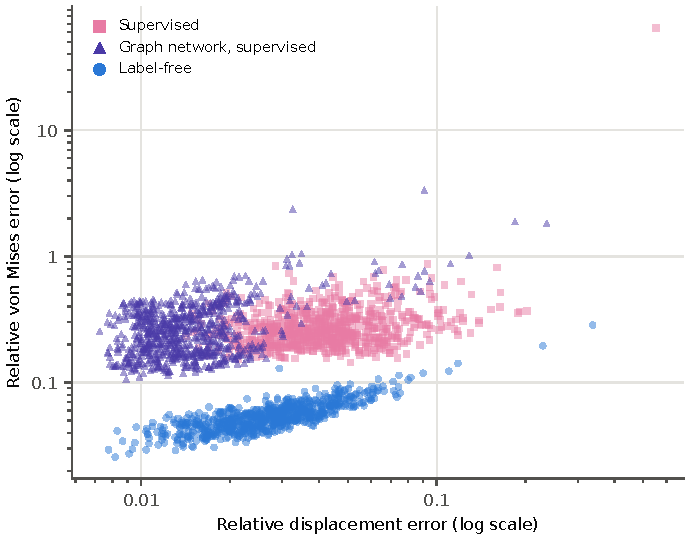
\includegraphics[width=0.72\linewidth]{generated/fig_disp_vs_stress.pdf}
\caption{Three dimensions, 1,024 labelled instances: relative displacement error against
relative von Mises error for every validation instance and seed (\numThreePairs{} points per
network). The graph network's points lie to the left of the label-free transformer's, at
lower displacement error, and above them, at higher stress error. The point at the top
right is instance No.~\numWorstIndex{} in seed \numThreeLabWorstSeed{}
(\cref{sec:results3d:same}).}
\label{fig:reverse}
\end{figure}

The graph network trained with labels had the lowest mean displacement error in
\cref{tab:3d}, \numThreeMgnDisp{}, \numThreeFreeOverMgnDisp{} times lower than the
label-free transformer's, and the label-free transformer was more accurate on every other
metric. The reversal holds on most instances individually (\cref{fig:reverse}). Compared
within each
seed, the graph network's displacement error was lower on \numMgnDispLowerMin{} to
\numMgnDispLowerMax{} of the instances, but its von Mises error was higher on
\numMgnVmHigher{} of the \numThreePairs{} instance-seed pairs, with a mean
\numThreeMgnOverFreeVm{} times higher, and its relative energy gap was higher on at least
\numMgnGapHigherMin{} of the instances in every seed. On \numMgnLowerDispHigherVm{} pairs
both held at once: a lower displacement error and a higher stress error. The peak stress
error, which compares a single value per load case, follows the pattern less closely: the
graph network's was the lower on \numMgnPeakLowerMin{} to \numMgnPeakLowerMax{} of the
instances, although its mean was \numThreeMgnOverFreePeak{} times higher.

Validation instance No.~\numWorstIndex{} in seed 0 (\cref{fig:field-worst}) shows the
pattern on one instance. The label-free transformer had the largest displacement error of
the three networks, \numWorstFreeDisp{}, and the most accurate stresses, with a von Mises
error of \numWorstFreeVm{} and a relative energy gap of \numWorstFreeGap{}. The supervised
transformer and the graph network had displacement errors of \numWorstLabDisp{} and
\numWorstMgnDisp{}, von Mises errors of \numWorstLabVm{} and \numWorstMgnVm{}, and relative
energy gaps of \numWorstLabGap{} and \numWorstMgnGap{}: both were more accurate in
displacement and worse than the zero field in energy. \Cref{fig:field-median} shows a
typical instance. \Cref{rem:rank} shows that such reversals are possible only when the
displacement errors differ by less than $\kappa^{1/2}$, and \cref{prop:stress} why the
energy, not the displacement, follows the stress.

\begin{figure}[tbp]
\centering
\pending{Field plot of validation instance No.~\numWorstIndex{}, seed 0: magnitude of the
displacement (top) and von Mises stress (bottom) of the reference solution and the three
networks, with the sign of $\Pi_h(u)$ for each network. The fields are exported on the
training machine together with the cost measurements of \cref{sec:cost}.}
\caption{Validation instance No.~\numWorstIndex{}, seed 0 (selection rule in
\cref{sec:methods:prereg}).}
\label{fig:field-worst}
\end{figure}

\begin{figure}[tbp]
\centering
\pending{Field plot of the validation instance with the median relative energy gap of the
label-free transformer, seed 0: von Mises stress of the reference solution, the
label-free transformer and the graph network.}
\caption{A typical validation instance, seed 0 (selection rule in
\cref{sec:methods:prereg}).}
\label{fig:field-median}
\end{figure}

\subsection{Failures and their detection}\label{sec:results3d:detection}

\begin{figure}[tbp]
\centering
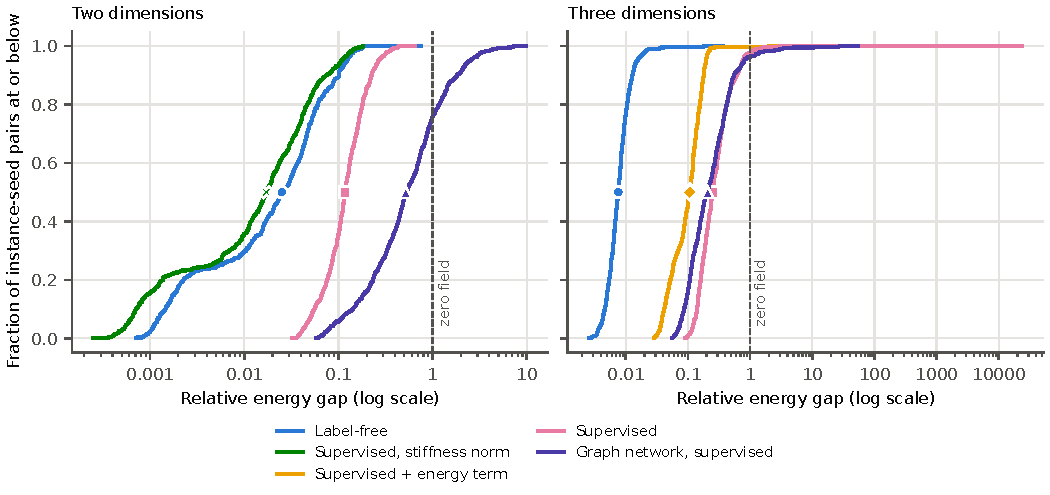
\includegraphics[width=\linewidth]{generated/fig_energy_gap.pdf}
\caption{Distribution of the relative energy gap over the \numThreePairs{} validation
instance-seed pairs, 1,024 labelled instances, in two dimensions (left) and three
dimensions (right). Markers show the medians; predictions to the right of the dashed line
are further from the solution, in the energy norm, than the zero field.}
\label{fig:energygap}
\end{figure}

\Cref{fig:energygap} shows the distribution of the relative energy gap. In three
dimensions the label-free transformer's median, \numThreeFreeGapMedian{}, was
\numThreeMedianRatioMin{} to \numThreeMedianRatioMax{} times lower than the supervised
networks' medians, and none of its \numThreePairs{} instance-seed predictions had a mean
relative energy gap above one. The supervised transformer had \numThreeLabWorse{} such
predictions, the supervised transformer with the energy term \numThreeAncWorse{} and the
graph network \numThreeMgnWorse{}. Per load case, the readings of
\cref{sec:transfer:amplitude} give the label-free transformer \numThreeFreeLoadWorse{}
prediction worse than the zero field among \numThreeFreeLoads{}.
\pending{Per-load-case counts for the supervised networks, from the energies exported on
the training machine.}

None of these failures needs a reference solution to be found. By \cref{cor:zero}, a load
case whose prediction is worse than the zero field is exactly one with $\Pi_h(u)>0$, which
is known as soon as the energy has been evaluated; by \cref{prop:amp}, rescaling by $\cstar$
turns it into a prediction no worse than the zero field. The check applies to any network,
however it was trained; for the label-free transformer the energy is also the training
objective.

\subsection{Label efficiency}\label{sec:results3d:labels}

In three dimensions (\cref{tab:labeleff,fig:labeleff}, right) the label-free
transformer's relative energy gap was lower than every supervised network's at every
budget, and its displacement error lower than both supervised transformers' at every
budget. The graph network reached a lower displacement error than the label-free
transformer with 1,024 labels, not with 64. The supervised transformer's relative energy
gap did not fall monotonically with the number of labels: its seed mean rose from 256 to
1,024 labels, through the single instance discussed in \cref{sec:results3d:same}.

\subsection{Pre-registered decisions}\label{sec:results3d:decisions}

The gate of this run combined three conditions as (a) and ((b) or (c))
(\cref{tab:criteria}). Condition (a)
is a sanity check on the supervised side: the supervised transformer with the energy term
must be at least \numGTwoSanityX{} times more accurate in displacement than the zero field
and better than both naive baselines. Condition (b) concerns the label-free transformer:
its displacement error within 10\% of the supervised transformer's with 1,024 labels, and
an advantage in relative energy gap of at least 40\% at every budget. Condition (c)
concerns transfer to the finer mesh.

Condition (b) was met with a wide margin: the label-free displacement error was
\numGTwoParity{} relative to the supervised one, and the smallest advantage in relative
energy gap was \numGTwoAdvMin{}. Condition (c) failed (\cref{sec:transfer}), and kill
condition KP4 withdrew the transfer claim. Condition (a) was met at 64, 256 and 1,024
labels, by factors of \numGTwoSanitySixtyFour{} to \numGTwoSanityMax{}, but not at 16
labels, where the factor was \numGTwoSanitySixteen{}. The amendment of
\cref{sec:methods:prereg} assessed (a) only from \numGTwoFloor{} labels on; under it the
gate read GO, under the registered form, which assesses every budget, NO-GO. Condition (a)
involves only the supervised networks and the baselines, whose results were known when the
amendment was written, so the change of reading was made with knowledge of its effect; it
was disclosed in the amendment itself, and the reference reading was computed and published
with the run. The conclusions of this paper rest on condition (b) and on the measurements
themselves, not on the gate's verdict.

\section{Transfer to a finer mesh}\label{sec:transfer}

\subsection{Zero-shot and few-shot}\label{sec:transfer:zeroshot}

% generated by scripts/make_cmame_material.py from the records; do not edit
\begin{table}[tbp]
\centering
\footnotesize
\setlength{\tabcolsep}{4pt}
\caption{Three-dimensional solids on the finer mesh ($l_c$ = 0.0374), never trained on. Zero-shot rows use the networks trained in-band; few-shot rows train, with labels, on the first 16 or on all of the 64 fine-mesh instances reserved for few-shot training.}
\label{tab:transfer}
\resizebox{\ifdim\width>\textwidth\textwidth\else\width\fi}{!}{%
\begin{tabular}{lccccc}
\toprule
Model & \shortstack{Displacement \\ error} & \shortstack{Relative \\ energy gap} & \shortstack{von Mises \\ error} & \shortstack{Peak stress \\ error} & \shortstack{Critical-region \\ recall} \\
\midrule
Label-free, zero-shot & 0.258 $\pm$ 0.045 & 0.306 $\pm$ 0.220 & 0.305 $\pm$ 0.063 & 0.769 $\pm$ 0.667 & 0.721 $\pm$ 0.006 \\
Supervised (1,024 labels), zero-shot & 0.257 $\pm$ 0.048 & 0.985 $\pm$ 0.267 & 0.537 $\pm$ 0.040 & 2.56 $\pm$ 1.39 & 0.462 $\pm$ 0.028 \\
Graph network (1,024 labels), zero-shot & 0.459 $\pm$ 0.010 & 16.3 $\pm$ 9.6 & 2.40 $\pm$ 0.84 & 11.6 $\pm$ 7.8 & 0.0610 $\pm$ 0.0083 \\
\midrule
Nearest-neighbour field & 0.401 & 4.98 & 1.55 & 3.61 & 0.232 \\
Scaled polynomial & 1.95 & 540 & 18.7 & 134 & 0.102 \\
\midrule
Label-free, then 16 fine-mesh labels & 0.0531 $\pm$ 0.0030 & 0.0702 $\pm$ 0.0112 & 0.166 $\pm$ 0.016 & 0.389 $\pm$ 0.061 & 0.715 $\pm$ 0.004 \\
Supervised from scratch, 16 fine-mesh labels & 0.799 $\pm$ 0.037 & 2.34 $\pm$ 1.25 & 1.07 $\pm$ 0.19 & 2.58 $\pm$ 1.23 & 0.116 $\pm$ 0.014 \\
Label-free, then 64 fine-mesh labels & 0.0298 $\pm$ 0.0020 & 0.0520 $\pm$ 0.0088 & 0.126 $\pm$ 0.018 & 0.272 $\pm$ 0.068 & 0.731 $\pm$ 0.014 \\
Supervised from scratch, 64 fine-mesh labels & 0.193 $\pm$ 0.076 & 13.2 $\pm$ 5.3 & 2.57 $\pm$ 0.47 & 8.94 $\pm$ 4.65 & 0.128 $\pm$ 0.043 \\
\bottomrule
\end{tabular}}

\smallskip
\begin{minipage}{\linewidth}\footnotesize\raggedright
256 fine-mesh evaluation instances (median 36,216 nodes), disjoint from the 64 instances reserved for few-shot training. Mean $\pm$ sample standard deviation over 3 seeds; the naive baselines are deterministic and built from the 1,024 in-band labelled instances.\par
In-band, the label-free network's displacement error is 0.0300; the zero-shot ratio is therefore 8.62.\par
Few-shot training runs 50 epochs at learning rate 1.5 $\times$ 10$^{-3}$ from the trained label-free network of the same seed, or from random initialisation (scratch); the few-shot comparison was pre-registered as reported only.
\end{minipage}
\end{table}


\Cref{tab:transfer} evaluates the networks trained in-band on the 256 fine-mesh evaluation
instances, meshed at $l_c=0.0374$, about half the in-band element size, which no network
had seen. None transferred. The label-free transformer's displacement error rose from
\numAmpInDisp{} in-band to \numFineFreeDisp{}, a factor of \numFineRatio{}; the
pre-registered criterion for transfer allowed \numFineWin{} and the kill condition KP4 was
triggered above \numFineKill{}, so the transfer claim was withdrawn. The supervised transformer
had almost the same displacement error, \numFineLabDisp{}, and the graph network
\numFineMgnDisp{}, worse than the nearest-neighbour field's \numFineKnnDisp{}. The
label-free transformer kept the lowest relative energy gap (\numFineFreeGap{} against
\numFineLabGap{} and \numFineMgnGap{}) and the lowest von Mises error (\numFineFreeVm{}
against \numFineLabVm{} and \numFineMgnVm{}).

Training on a few labelled fine-mesh instances, starting from the trained label-free
network, was
pre-registered as a reported comparison without a criterion. With 64 such instances the
displacement error returned to the in-band level, \numFewSixtyFourDisp{}, and with 16 it
was \numFewSixteenDisp{}, against \numFewSixtyFourScratchDisp{} and
\numFewSixteenScratchDisp{} when the same network was trained from scratch on the same
instances. The relative energy gap, von Mises error and peak stress error did not recover
as far: with 64 instances they remained \numFewFactorMin{} to \numFewFactorMax{} times their
in-band values.

\subsection{On the finer mesh, most of the label-free error is an error of
amplitude}\label{sec:transfer:amplitude}

% generated by scripts/make_cmame_material.py from the records; do not edit
\begin{table}[tbp]
\centering
\footnotesize
\setlength{\tabcolsep}{4pt}
\caption{Post hoc, three-dimensional: errors before and after scaling each prediction by its energy-optimal amplitude $c^*$, in-band and on the finer mesh (zero-shot).}
\label{tab:amplitude}
\resizebox{\ifdim\width>\textwidth\textwidth\else\width\fi}{!}{%
\begin{tabular}{lccccccc}
\toprule
Network & \shortstack{In-band \\ displacement} & \shortstack{In-band \\ with $c^*$} & \shortstack{Fine displacement \\ (zero-shot)} & \shortstack{Fine \\ with $c^*$} & \shortstack{Fine relative \\ energy gap (median)} & \shortstack{Fine \\ with $c^*$} & \shortstack{Median $c^*$ \\ (fine)} \\
\midrule
Transformer & 0.0300 $\pm$ 0.0028 & 0.0142 $\pm$ 0.0032 & 0.258 $\pm$ 0.045 & 0.0832 $\pm$ 0.0158 & 0.0911 $\pm$ 0.0177 & 0.0418 $\pm$ 0.0031 & 1.23 $\pm$ 0.08 \\
Bottleneck, M = 512 & 0.106 $\pm$ 0.051 & 0.0393 $\pm$ 0.0243 & 0.463 $\pm$ 0.082 & 0.124 $\pm$ 0.039 & 0.258 $\pm$ 0.075 & 0.0904 $\pm$ 0.0405 & 1.73 $\pm$ 0.42 \\
Bottleneck, M = 1,024 & 0.0892 $\pm$ 0.0096 & 0.0292 $\pm$ 0.0049 & 0.574 $\pm$ 0.059 & 0.126 $\pm$ 0.037 & 0.263 $\pm$ 0.037 & 0.0717 $\pm$ 0.0326 & 1.77 $\pm$ 0.28 \\
\bottomrule
\end{tabular}}

\smallskip
\begin{minipage}{\linewidth}\footnotesize\raggedright
$c^*$ = $F^\top u / (u^\top K u)$, per load case: the energy-optimal amplitude of the prediction $u$ on the evaluated mesh, from that mesh's stiffness matrix $K$ and load vector $F$ (no labels, no solve). Scaling by $c^*$ never increases the error in the energy norm (it did not in any of the 4,608 instance-seed evaluations measured). In-band median $c^*$: 1.00 (transformer), 1.00 (M = 512), 1.00 (M = 1,024).\par
Seeds per network: 3; seed mean $\pm$ sample SD of the per-seed mean over instances (relative energy gap: per-seed median). In-band: the 256 validation instances; fine: 256 instances at $l_c$ = 0.0374, never trained on. The columns without $c^*$ reproduce the runs' own per-instance arrays: the transformer's exactly, the bottleneck's to a relative 0.011 at most; the bottleneck run's own two evaluations of the same trained networks (in-band) differ by up to 0.003, the transformer run's not at all.\par
Mean fine relative energy gap over instances (a heavy tail), as trained $\rightarrow$ with $c^*$: transformer: 0.306 $\rightarrow$ 0.0670; M = 512: 0.295 $\rightarrow$ 0.106; M = 1,024: 0.590 $\rightarrow$ 0.0984.\par
Measured after the runs; no verdict is revisited.
\end{minipage}
\end{table}


Rescaling each prediction by its energy-optimal amplitude $\cstar$ (\cref{prop:amp}),
which needs no label and no solve, separates errors of amplitude from errors of shape. We
measured it after the runs, on the stored networks (\cref{tab:amplitude}); no verdict was
revisited. On the finer mesh the median $\cstar$ of the label-free transformer was
\numAmpFineCstar{}, against \numAmpInCstar{} in-band: its predictions were too small.
Rescaling lowered its fine-mesh displacement error from \numAmpFineDisp{} to
\numAmpFineDispC{}, by \numAmpFineRedMin{} to \numAmpFineRedMax{} in each seed, and the
median relative energy gap from \numAmpFineGapMedian{} to \numAmpFineGapMedianC{}. In-band
it also helped, from \numAmpInDisp{} to \numAmpInDispC{} in displacement and from
\numAmpInGap{} to \numAmpInGapC{} in mean relative energy gap. Measured as KP4 measures
transfer, with $\cstar$ applied on both meshes, the ratio of fine-mesh to in-band
displacement error fell from \numFineRatio{} to \numAmpRatioBoth{}; with $\cstar$ applied
on the finer mesh only it was \numAmpRatioFineOnly{}. Rescaling removes most of the error
but not the failure to transfer.

% generated by scripts/make_cmame_material.py from the records; do not edit
\begin{table}[tbp]
\centering
\footnotesize
\setlength{\tabcolsep}{4pt}
\caption{Post hoc, three-dimensional: the energy-optimal amplitude $c_b$ of the four load cases of an instance together, on fixed geometries and loads meshed at four mesh sizes $l_c$.}
\label{tab:remesh}
\resizebox{\ifdim\width>\textwidth\textwidth\else\width\fi}{!}{%
\begin{tabular}{lcccc}
\toprule
Network & $l_c$ = 0.0906 & $l_c$ = 0.0742 & $l_c$ = 0.0579 & \shortstack{$l_c$ = 0.0374 \\ (fine)} \\
\midrule
Transformer & 0.98 $\pm$ 0.00 & 1.00 $\pm$ 0.01 & 1.01 $\pm$ 0.00 & 1.27 $\pm$ 0.08 \\
Bottleneck, M = 512 & 0.91 $\pm$ 0.04 & 1.00 $\pm$ 0.02 & 1.14 $\pm$ 0.09 & 1.96 $\pm$ 0.46 \\
Bottleneck, M = 1,024 & 0.94 $\pm$ 0.01 & 1.01 $\pm$ 0.01 & 1.14 $\pm$ 0.02 & 1.99 $\pm$ 0.35 \\
\bottomrule
\end{tabular}}

\smallskip
\begin{minipage}{\linewidth}\footnotesize\raggedright
16 fresh geometries, each meshed at the 4 $l_c$ with identical geometry and loads, so only the mesh changes; every mesh evaluated by every seed. $c_b$: the single energy-optimal amplitude of all four load cases of an instance (label-free, \cref{sec:transfer:amplitude}); median over the geometries, then seed mean $\pm$ sample SD. Training range: $l_c$ = 0.0579--0.0906.\par
The largest nodal load over the four load cases, by which both networks multiply their output, relative to $l_c$ = 0.0906, at $l_c$ = 0.0742 / 0.0579 / 0.0374: 0.705 / 0.430 / 0.186; for comparison ($l_c$ / 0.0906)$^2$: 0.671 / 0.408 / 0.170.\par
Predicted energy norm relative to $l_c$ = 0.0906 (label-free), seed means, $l_c$ = 0.0742 / 0.0579 / 0.0374: transformer: 0.99 / 0.98 / 0.75; M = 512: 0.90 / 0.82 / 0.50; M = 1,024: 0.93 / 0.83 / 0.49.\par
Measured after the runs.
\end{minipage}
\end{table}


Why the amplitude is wrong on the finer mesh is suggested by \cref{tab:remesh}, also
measured after the runs: \numRemeshGeometries{} new geometries, each meshed at four
characteristic lengths with the same loads, so that only the mesh changes. For each mesh
we computed the single energy-optimal amplitude of all four load cases,
$c_b=\sum_jF_j^{\top}u_j/\sum_ju_j^{\top}Ku_j$, the counterpart of \eqref{eq:cstar} for
the sum of their energies. Over the training range the median $c_b$ of the label-free
transformer stayed within \numRemeshInDev{} of one, and at $l_c=0.0374$ it was
\numRemeshFine{}. The largest nodal load $F_{\max}$, by which the output is multiplied
(\cref{sec:methods:networks}), shrinks with the element size, roughly as $l_c^2$ for the
face tractions, whereas the solution does not depend on the mesh; a finer mesh therefore
asks the network for a larger output than any it produced in training. We have not tested
this explanation causally. It agrees with the two-dimensional observation of
\cref{sec:results2d:other}, where the output was not multiplied by $F_{\max}$ and networks
trained on meshes \numCoarsenLow{} and \numCoarsenHigh{} times coarser lost little accuracy
on the original meshes; but the errors of those networks were probably dominated by the
missing load amplitude (\cref{sec:results2d:julyaccuracy}), so the contrast is suggestive
only. A separate pre-registered
study, outside the scope of this paper, tests an output scale that does not depend on the
mesh. \Cref{fig:field-fine} shows a typical fine-mesh prediction before and after the
rescaling: the prediction has the shape of the solution and too small an amplitude.

\begin{figure}[tbp]
\centering
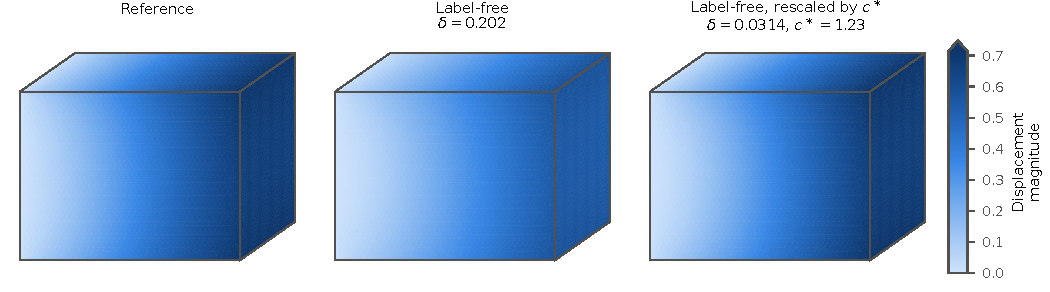
\includegraphics[width=\linewidth]{generated/fig_field_fine.pdf}
\caption{A typical fine-mesh instance, the one with the median displacement error of the
label-free transformer, seed 0, under the \numFigFineLoad{} (selection rules in
\cref{sec:methods:prereg}). Magnitude of the displacement of the reference solution, of the
label-free prediction and of that prediction rescaled by $\cstar$ \eqref{eq:cstar}, on one
colour scale set by the reference and displayed as in \cref{fig:field-worst}; above each
prediction, its relative displacement error $\delta$ on this load case and, for the rescaled
one, $\cstar$.}
\label{fig:field-fine}
\end{figure}

\section{Computational cost}\label{sec:cost}

\subsection{Labels}\label{sec:cost:labels}

In two dimensions the comparison of \cref{sec:results2d} used \numCmSolves{} solves,
\numCmSolvesVal{} for the 256 validation instances and \numCmSolvesTrain{} for the 1,024
labelled training instances, four load cases each; the run of 16 July 2026 used the same
labelled instances and a further \numTwoSolvesRun{} solves for the coarsened validation sets
of \cref{sec:results2d:other}. In three dimensions the comparison consumed
\numThreeSolves{}:
\numThreeTrainSolves{} for the 1,024 labelled training instances, \numThreeFewSolves{} for
the 64 fine-mesh instances reserved for few-shot training and \numThreeEvalSolves{} for the in-band and fine-mesh
validation sets. The validation solves are needed to evaluate any method; the training
solves are the price of supervision, and the label-free transformer needed none of them.

\subsection{Training}\label{sec:cost:training}

Label-free training of the three-dimensional transformer took \numTimeThreeSeed{} h per
seed on one NVIDIA GeForce RTX 5090, for 204,800 steps; the supervised transformer costs
the same per step, plus its labels. Full self-attention over all nodes dominates this cost
and grows with the square of the number of nodes: one training step took
\numEtwoTransformerFineStep{} s on a fine-mesh instance of \numEtwoNodesFine{} nodes. In
two dimensions, with the later code (\cref{sec:methods:networks}), three label-free seeds
trained in parallel on one GPU of the same type took \numTimeTwoParallel{}.

To reduce the cost of attention we tested, under a separate pre-registration, a
token-bottleneck network that pools the nodes into $M=512$ or $M=1{,}024$ tokens seeded by
farthest-point sampling, applies attention to the tokens only, and decodes each node from
a smooth blend of its six nearest tokens; it was trained on the energy alone, with every
other setting as for the transformer (\cref{tab:e2,fig:e2}). It trained
\numTimeBottleneckSpeedup{} times faster per seed (\numTimeBottleneckSeedMin{} h against
\numTimeThreeSeed{} h), but it was less accurate: its in-band relative energy gap was
\numEtwoGapMin{} to \numEtwoGapMax{} times the transformer's and its zero-shot fine-mesh
displacement error \numEtwoFineMin{} to \numEtwoFineMax{} times. Both variants were
dropped under their pre-registered accuracy criterion (\cref{tab:criteria}).

% generated by scripts/make_cmame_material.py from the records; do not edit
\begin{table}[tbp]
\centering
\footnotesize
\setlength{\tabcolsep}{4pt}
\caption{Token bottleneck against the transformer with one token per node, both trained on the energy alone with the same corpus, split, seeds and schedule (3D).}
\label{tab:e2}
\resizebox{\ifdim\width>\textwidth\textwidth\else\width\fi}{!}{%
\begin{tabular}{lccccc}
\toprule
Network & \shortstack{In-band \\ displacement} & \shortstack{In-band relative \\ energy gap} & \shortstack{Fine displacement \\ (zero-shot)} & \shortstack{Step (ms), \\ 12,318 nodes} & \shortstack{Step (ms), \\ 41,367 nodes} \\
\midrule
Transformer & 0.0300 $\pm$ 0.0028 & 0.00912 $\pm$ 0.00228 & 0.258 $\pm$ 0.045 & 1,415 & 14,795 \\
Bottleneck, M = 512 & 0.106 $\pm$ 0.051 & 0.0348 $\pm$ 0.0226 & 0.463 $\pm$ 0.082 & 27.8 & 49.2 \\
Bottleneck, M = 1,024 & 0.0892 $\pm$ 0.0096 & 0.0258 $\pm$ 0.0051 & 0.574 $\pm$ 0.059 & 36.9 & 47.5 \\
\bottomrule
\end{tabular}}

\smallskip
\begin{minipage}{\linewidth}\footnotesize\raggedright
M = 512: accuracy criterion, in-band relative energy gap +280.9\% (resolution 287\%), fine displacement +79.1\% (resolution 42\%; triggered); speed criterion, fine-mesh step 0.049 s against the 2.0 s limit: not triggered. Outcome: dropped.\par
M = 1,024: accuracy criterion, in-band relative energy gap +183.3\% (resolution 70\%; triggered), fine displacement +122.0\% (resolution 33\%; triggered); speed criterion, fine-mesh step 0.047 s against the 2.0 s limit: not triggered. Outcome: dropped.\par
Seeds per network: 3; seed mean $\pm$ sample SD. In-band: the 256 validation instances ($l_c$ = 0.0579--0.0906; the benchmark instances at the two ends of this range have 12,318 and 3,774 nodes); fine: 256 instances at $l_c$ = 0.0374 (41,367 nodes in the benchmark), never trained on. Errors are relative displacement error and relative energy gap.\par
Step time: one label-free training step on one instance of the stated size, NVIDIA GeForce RTX 5090, TF32 on, from a dedicated benchmark (bottleneck: the median over three repetitions of the time of 110 steps minus that of 10 steps, divided by 100, which removes the set-up time; transformer: a single timed step, its set-up included, the mean of its two benchmark measurements, 1,408 / 1,422 ms and 14,793 / 14,798 ms).\par
Resolution: the pre-registered max(10\%, 2 $\times$ SE$_\mathrm{rel}$), where SE$_\mathrm{rel}$ = $(s_\mathrm{T}^2/3 + s_\mathrm{B}^2/3)^{1/2}$ divided by the transformer's seed mean, with $s_\mathrm{T}$ and $s_\mathrm{B}$ the sample standard deviations of the two networks over the three seeds.
\end{minipage}
\end{table}


\begin{figure}[tbp]
\centering
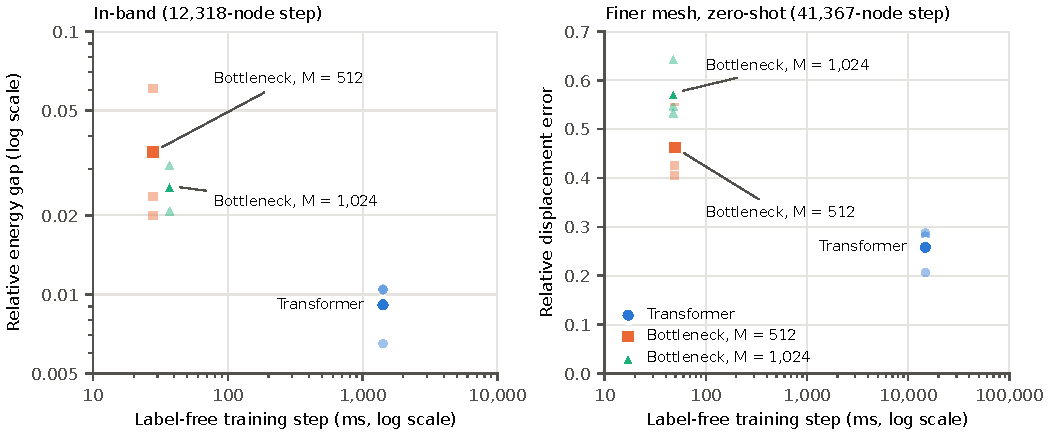
\includegraphics[width=\linewidth]{generated/fig_e2_cost_accuracy.pdf}
\caption{Cost against accuracy of the label-free transformer and the token bottleneck
(three dimensions, three seeds each; faint markers are seeds, ringed markers seed means).
Left: in-band relative energy gap against the time of one training step on an in-band
instance. Right: zero-shot fine-mesh displacement error against the time of one step on a
fine-mesh instance.}
\label{fig:e2}
\end{figure}

\subsection{Inference and solving}\label{sec:cost:inference}

\pending{A cost table: on the training machine and on the same validation and fine-mesh
instances, the time of surrogate inference (first call and repeated calls) against a
sparse direct solve, conjugate gradients from zero, conjugate gradients from the
prediction, and conjugate gradients stopped once the energy error of the iterate reaches
that of the prediction, with and without the rescaling of \cref{prop:amp}, together with
the surrogate's accuracy on those instances. The last two use the reference solution to
decide when to stop, so they give a lower bound on the time conjugate gradients need to
match the surrogate.}

\section{Discussion}\label{sec:discussion}

% DRAFT: to be completed after the field plots and the cost table are in, and after the
% full texts of the flagged related works have been read.

\paragraph{What the comparison measures}
By \cref{cor:training}, training on the energy is supervised regression in the stiffness
norm. The labels of the supervised networks carry no information that the assembled $K$
and $F$ do not, so the comparisons of \cref{sec:results2d,sec:results3d} are between two
losses: the stiffness-norm error, which can be evaluated without a solve, and the relative
displacement error, the usual supervised loss, which cannot. A supervised network trained
on the stiffness-norm error would share the label-free network's objective while paying for
the labels; we did not train one. The claim of this paper is therefore not that labels are
uninformative, but that the norm in which one can train without labels is the one that
controls the stresses, and that supervised training in the usual displacement norm does
not control them.

\paragraph{Why the label-free network's stresses are accurate}
By \cref{cor:training,prop:stress}, the label-free objective is, up to a constant, the
compliance-weighted mean-square error of the stress field. The supervised networks were
trained on the relative Euclidean error of the displacement, which weights all eigenmodes
of the stiffness matrix equally and so under-weights, relative to the energy norm, the
stiff modes that carry the strains (\cref{sec:theory:metrics}). A supervised network can
therefore reach a small displacement error with an error rich in stiff modes, and a large
stress error; instance No.~\numWorstIndex{} in seed 0 (\cref{sec:results3d:reverse}) is an
example, with a displacement error of \numWorstLabDisp{} and a relative energy gap of
\numWorstLabGap{}. The
energy term of the supervised transformer is a partial remedy: it added the stress-weighted
signal and removed most of the large failures, but on the same instances the label-free
transformer, which receives only that signal, was more accurate still.

\paragraph{The graph network}
The graph network had the lowest displacement error and among the largest stress errors.
On an instance where its displacement error is the lower and its energy-norm error the
higher, its error has the larger Rayleigh quotient $e^{\top}Ke/e^{\top}e$: relatively more
weight in stiff modes, as for an error that varies rapidly from node to node
(\cref{rem:rank}). We have not measured the spectral content of the errors; the field
plots of \cref{fig:field-worst,fig:field-median}, pending, will illustrate it. The observation matters for evaluation more than for the graph
network itself: a ranking of surrogates by displacement error alone can invert their
ranking by stress, the quantity on which design decisions usually depend.

\paragraph{The energy in deployment}
\Cref{cor:zero,prop:amp} give every surrogate, however it was trained, a check and a
repair that need only the assembled $K$ and $F$: the sign of $\Pi_h(u)$ flags a prediction
worse than the zero field, the difference of energies ranks the predictions of several
surrogates for the same instance exactly by their energy-norm errors, and the rescaling by
$\cstar$, which costs nothing once $\Pi_h(u)$ is known, removes any error of amplitude and
never increases the error in the energy norm. Every supervised network of
\cref{tab:2d,tab:3d} returned predictions that the check would have flagged; so, in
\numTwoFreeWorse{} of its \numTwoPairs{} instance-seed predictions, did the
two-dimensional label-free network.

\paragraph{Warm starts}
The label-free prediction did not shorten conjugate gradients to a relative residual of
\numKfiveTol{} in two dimensions (\cref{sec:results2d:decisions}), whereas the pretrain
finite element method has been reported to accelerate the warm-start stage of the solver by
up to an order of magnitude \cite{Wang2026PretrainFEM}, and neural operator warm starts
have been reported to accelerate iterative solvers \cite{Eshaghi2026NOWS}. \Cref{cor:warm}
suggests why the two kinds of result need not conflict: a warm start lowers the iteration
bound by a number of iterations set by its own accuracy, so the share of the run it can
save grows as the tolerance loosens and shrinks as it tightens, and a residual-based stop
can hide part of it (\cref{rem:residual}). Reported warm-start speed-ups are therefore
comparable only when the tolerance, the stopping test and the preconditioner are stated
with them. The comparison of solver settings with \cite{Wang2026PretrainFEM,Eshaghi2026NOWS}
is to be completed after their full texts have been read.

\paragraph{Transfer}
No network transferred to the finer mesh, and the readings of \cref{sec:transfer} point at
the output scaling: the network's output is multiplied by the largest nodal load, which
depends on the mesh, while the solution does not. The two-dimensional networks, whose
output was not scaled in this way, lost little accuracy on meshes \numCoarsenLow{} and
\numCoarsenHigh{} times finer, although that evidence is weak (\cref{sec:transfer}). A
separate pre-registered study tests an output scale independent of the mesh. Until it
reports, the label-free transformer of this paper should be regarded as valid within the
range of mesh sizes it was trained on.

\paragraph{Limitations}
The study is restricted to linear elastostatics, where \cref{lem:exact} is exact; one
family of geometries and one set of four load cases per dimension; and three seeds per
network. The two-dimensional runs of \cref{sec:results2d} used code that could not recover
the absolute load amplitude, and their supervised networks were not repeated with the later
code; their pre-registration documents were committed to the repository only after the runs
(\cref{sec:methods:prereg}). The scope of this paper, the energy objective without the
joint-embedding term that a pre-registered comparison kept, was chosen after that
comparison (\ref{app:prereg}). The
three-dimensional gate was amended after the initial run (\ref{app:prereg}), and both
readings are reported. The supervised baselines were trained on the relative displacement
error, the usual choice, and no supervised network was trained on the stiffness-norm error.
The reported von Mises error weights elements equally, so \cref{prop:stress} explains it
rather than bounds it. The inference cost (\cref{sec:cost:inference}), the field plots and
the per-load-case failure counts of the supervised networks are pending. No network
transferred to a substantially finer mesh.

\paragraph{Outlook}
The construction extends wherever each step of a computation is a convex minimisation. In
linear dynamics, every implicit step of a Newmark-type integrator solves a symmetric
positive definite system whose effective stiffness combines the stiffness, mass and
damping matrices, and \cref{lem:exact} holds step by step \cite{CaoSong2026}. Incremental
variational formulations of dissipative materials \cite{OrtizStainier1999} and variational
integrators \cite{MarsdenWest2001} write each step of a nonlinear history as the
minimisation of an incremental potential. There the energy remains a label-free training
objective, although the energy gap is no longer a squared norm, and the counterparts of
\cref{prop:amp,cor:zero} remain to be worked out. These are the problems in which a solve
may be expensive enough for label-free training to pay for itself.

\section{Conclusion}\label{sec:conclusion}

For linear elastostatics, the assembled discrete potential energy is an exact label-free
training objective: minimising it is supervised regression in the stiffness norm, which
measures the strain energy of the stress error, and it needs no solve. The same identity
makes the energy an evaluation metric that follows the stress rather than the displacement,
and a failure detector: the sign of the energy of a prediction tells whether it is worse
than the zero field, and a closed-form rescaling ensures that it is not. In
pre-registered comparisons on three-dimensional tetrahedral meshes, a transformer trained
on the energy alone was more accurate on every metric than the same transformer trained on
the solutions of the same instances, and a supervised graph network with lower
displacement errors had several times larger stress errors, so that displacement error
ranked the two in the opposite order to stress error. In two dimensions the label-free
network had a larger displacement error than the supervised one and smaller energy and stress
errors. Trained on the stiffness-norm error instead of the displacement error, with the same
labels, the supervised network halved its von Mises error, as pre-registered, and its errors
lay lower in the spectrum of the stiffness matrix, as measured afterwards: with the labels
fixed, the norm of the loss decided the accuracy of the stresses. In two dimensions, warm
starts from a label-free prediction did not shorten conjugate gradients to a tight
tolerance. In three dimensions no network transferred to a substantially finer mesh without
retraining, although a label-free rescaling removed most of the label-free network's error
there.
These limits, and the criteria that were not met, are reported with the results.


\appendix
\section{Pre-registration record and deviations}\label{app:prereg}
\setcounter{table}{0}\setcounter{figure}{0}\setcounter{equation}{0}

% generated by scripts/make_cmame_material.py from the records; do not edit
\begingroup\small
\begin{longtable}{@{}>{\raggedright\arraybackslash}p{0.14\linewidth}>{\raggedright\arraybackslash}p{0.42\linewidth}>{\raggedright\arraybackslash}p{0.21\linewidth}>{\raggedright\arraybackslash}p{0.11\linewidth}@{}}
\caption{Every pre-registered criterion of the runs reported here, with its outcome.}\label{tab:criteria}\\
\toprule
Run & Criterion & Measured & Outcome \\
\midrule
\endfirsthead
\caption[]{Every pre-registered criterion of the runs reported here, with its outcome. (continued)}\\
\toprule
Run & Criterion & Measured & Outcome \\
\midrule
\endhead
\bottomrule
\endfoot
2D, 16 July 2026 & G1$'$ (a), energy-term sub-experiment (separately trained networks): supervised + energy term at least 3 times better than the zero field in displacement, and better than the 3 naive baselines fitted on 1,024 labelled instances, at every budget & 4.5--6.1 times; naive baselines beaten at every budget & met \\
 & G1$'$ (b), Tables 1 and 2, 64 labels: the energy term lowers the relative energy gap by $\geq$ 50\% and the von Mises error by $\geq$ 25\% & 78.7\%, 65.4\% & met \\
 & G1$'$ (c), Tables 1 and 2, 64 labels: label-free, then supervised beats supervised by $\geq$ 10\% in relative energy gap or $\geq$ 5\% in displacement & 92.6\%, 2.0\% & met \\
 & Gate G1$'$ = (a) and (b) and (c) &  & GO \\
 & K1, energy-term sub-experiment: the better of the fixed and the gradient-scaled energy term lowers the relative energy gap by $<$ 25\% at every budget & 98.0\% / 94.4\% / 90.6\% / 74.0\% & not triggered \\
 & K2, Table 1: label-free displacement error $>$ 30\% above supervised, 1,024 labels & +3.6\% & not triggered \\
 & C1-advantage, Table 2: label-free relative energy-gap advantage over supervised $<$ 40\% at every budget & 98.7\% / 97.0\% / 93.5\% / 80.4\% & not triggered \\
 & K4: a latent-space regulariser raises the standardised effective rank of the latent vectors by $\leq$ 1.5 times & 1.70 times & not triggered \\
 & K5: conjugate gradients from the prediction of a label-free network (64 validation instances) save $<$ 20\% of the iterations from zero & $-$0.9\% & triggered \\
 & K6: a cross-resolution invariance term shrinks the transfer gap by $<$ 10\% at coarsening 2.5 & $-$23.7\% & triggered \\
 & E6 (alignment): within-geometry rank correlation of latent and solution distances $<$ 0.3 & 0.730 & not triggered \\
 & C5: any pre-registered check of the conditioning bound, the modewise identity or the conjugate-gradient bound violated & none & not triggered \\
\midrule
2D, 31 July 2026 & K3: a self-supervised joint-embedding term added to label-free pretraining changes the displacement error and the relative energy gap of the transformer, fine-tuned with 16, 64 and 256 labels, by less than 3\% at every budget (if triggered, the term is dropped) & change with the term, 16 / 64 / 256 labels: displacement $-$13.5\% / $-$0.5\% / +2.6\%; relative energy gap $-$48.4\% / +92.5\% / $-$16.4\% (positive: more accurate) & not triggered \\
\midrule
3D, 21 September 2026 & Initial run: gate G2 and kill conditions as registered; the label-free objective was defective (deviation D14) & (a), (b), (c) not met; KP1, KP2, KP4 triggered & NO-GO \\
3D, 22 September 2026 & Pilot of the amendment: label-free displacement error after 20 epochs $<$ 0.90 & 0.309 & met \\
3D, 28 September 2026 & G2 (a), budgets $\geq$ 64 (amendment), Table 2: supervised + energy term at least 3 times better than the zero field in displacement, and better than both naive baselines & 3.9 / 12.0 / 21.3 times; naive beaten & met \\
 & G2 (a), every budget (the registered form, reported for reference) & 2.71 times at 16 labels & not met \\
 & G2 (b), Tables 2 and 3: label-free displacement error within +10\% of supervised at 1,024 labels, and relative energy-gap advantage $\geq$ 40\% at every budget & $-$36.3\%; 99.95\% / 99.85\% / 98.86\% / 99.97\% & met \\
 & G2 (c), Table 4: finer mesh, zero-shot displacement error $\leq$ 1.25 times in-band, and better than both naive baselines & 8.62 times; best naive 0.401 against 0.258 & not met \\
 & Gate G2 = (a) and ((b) or (c)), amended &  & GO \\
 & Gate G2, registered form (reference) &  & NO-GO \\
 & KP1: supervised (1,024 labels) better than label-free by $>$ 10\% in displacement & $-$36.3\% & not triggered \\
 & KP2: relative energy-gap advantage $<$ 40\% at any budget & minimum 98.9\% & not triggered \\
 & KP3: the energy term lowers the relative energy gap by $<$ 25\% at every budget & +96.6\% / +85.7\% / $-$20.7\% / +99.6\% & not triggered \\
 & KP4: finer mesh, zero-shot displacement error $>$ 1.5 times in-band, or a naive baseline better & 8.62 times & triggered \\
 & KP5: any pre-registered check of the conditioning bound, the modewise identity or the conjugate-gradient bound violated & none & not triggered \\
 & KP6 (alignment): within-geometry rank correlation of latent and solution distances $<$ 0.3 & 0.827 & not triggered \\
\midrule
2D, 29 September 2026 & Latent regularisation, K1: relative change of the displacement error or of the relative energy gap beyond the resolution & within the resolution & not triggered \\
 & Latent regularisation, K2: the separation does not rise in any seed & rose in every seed & not triggered \\
 & Latent regularisation, GO: separation raised by $\geq$ 0.02 in every seed & +0.009 / +0.014 / +0.002 & NO-GO \\
\midrule
3D, 30 September 2026 & Token bottleneck, M = 512, K1: in-band relative energy gap or finer-mesh displacement error worse than the transformer's by more than the resolution & +280.9\% (resolution 287.2\%), +79.1\% (resolution 41.9\%) & triggered \\
 & Token bottleneck, M = 512, K2: finer-mesh training step longer than 2 s & 0.049 s & not triggered \\
 & Token bottleneck, M = 512: outcome &  & dropped \\
 & Token bottleneck, M = 1,024, K1: in-band relative energy gap or finer-mesh displacement error worse than the transformer's by more than the resolution & +183.3\% (resolution 70.5\%), +122.0\% (resolution 33.3\%) & triggered \\
 & Token bottleneck, M = 1,024, K2: finer-mesh training step longer than 2 s & 0.047 s & not triggered \\
 & Token bottleneck, M = 1,024: outcome &  & dropped \\
\end{longtable}
\endgroup
\vspace{-\smallskipamount}
\noindent\begin{minipage}{\linewidth}\footnotesize\raggedright
Labels are those of the pre-registration documents, each of which numbers its own criteria. Gates (G1$'$, G2) decide whether the study proceeds to its next stage. Kill conditions withdraw a claim, or abandon a component, when triggered: in two dimensions K1--K6, C1-advantage (the claimed advantage in relative energy gap), C5 (the pre-registered checks of \cref{sec:theory:checks}) and E6 (latent alignment); in three dimensions KP1--KP6, with KP5 the counterpart of C5. The latent-regularisation and token-bottleneck runs number their criteria afresh, with the meanings given here. A criterion reads the trained networks of the tables it names; the energy-term sub-experiment of the 2D run of 16 July 2026 trained its own supervised networks with and without the energy term, with the same configuration. K4, E6 and KP6 concern latent representations, which this paper does not use. Standardised effective rank: the participation ratio of the eigenvalues of the covariance of the latent vectors, each dimension standardised. The 3D amendment, the deviations and the joint-embedding term are described below, the latent regularisation in \ref{app:e1} and the token bottleneck in \cref{sec:cost:training}.
\end{minipage}
\par\medskip


\Cref{tab:criteria} lists every criterion fixed in advance for the runs reported in this
paper, with the value measured and the outcome as recorded by the code at the time. The
two-dimensional pre-registration also retired, before its run, an earlier criterion (a
displacement improvement of at least 10\% from the energy term with 64 labels) that an
earlier run had already answered in the negative; the run of 16 July 2026 measured
\numGOneRetired{} with the fixed-weight form of the energy term, and the criterion played no
part in its decisions. The following departures from the plans bear on the results. They
are recorded in the repository's list of deviations and its provenance note, except the
remark at the end of the paragraph on the energy term, which was noticed while this paper
was written.

\paragraph{Deviation D14}
The initial three-dimensional run (21 September 2026) completed its registered protocol and
read NO-GO, with conditions (a), (b) and (c) of its gate unmet and kill conditions KP1,
KP2 and KP4 triggered. After the verdict, its label-free networks were found to have a
displacement error of \numDfourteenDisp{} and a relative energy gap of
\numDfourteenGap{}, identical to five decimals across seeds and consistent with predicting
the solution scaled by $\alpha=\numDfourteenAlpha{}$ (displacement error $1-\alpha$,
relative energy gap $(1-\alpha)^2$). The cause was in the code: inference multiplied the
decoded field by $F_{\max}$, the label-free objective scored it without that factor, and on
this corpus $F_{\max}\approx\alpha$. The fix gives the network one decoding path, used by
the objective and by inference, with a test that fails on the registered code. The
supervised networks, which are trained and evaluated through the inference path, were not
affected. The verdict of the initial run stands as recorded. A pre-registered amendment then
repeated everything that depended on the label-free objective: the label-free networks,
their fine-tuning on the finer mesh and the latent-alignment criterion read from them. It
reused the 30 trained supervised networks and the 6 networks trained from scratch on the
fine mesh, each checked against its recorded SHA-256 hash, and it required a short pilot
run first: one seed, 20 epochs, which had to bring the displacement error below
\numPilotLimit{} and reached \numPilotDisp{}. A first version of the amendment was
registered and withdrawn on the same day, before any run, because the audit of its
execution path had not been completed; the second version was registered after the audit.
The amended run (28 September 2026) was executed once, without interruption.

\paragraph{The sanity condition of the three-dimensional gate}
Condition (a) of the three-dimensional gate required the supervised transformer with the
energy term to be at least three times more accurate in displacement than the zero field,
and better than both naive baselines, at every budget. In the initial run it failed at 16
labels (\numGTwoSanitySixteen{} times), independently of D14. The amendment, written with
this result known, assessed condition (a) only from the decision budget of 64 labels, where
it was met by factors of \numGTwoSanitySixtyFour{} to \numGTwoSanityMax{}. Its stated
rationale is that the factor of three had been calibrated on the two-dimensional family,
and that on the three-dimensional family the supervised network itself sits below it with
16 labels and above it from 64 labels on. In two dimensions the condition had read the
networks of the energy-term sub-experiment, which met it at every budget; the networks of
\cref{tab:labeleff} would not have met it with 16 labels (\numGOneSanityTableSixteen{}
times), because of the scatter described in \cref{sec:results2d:labels}. The amendment
declared the change as made after the fact and required the original form to be computed
and reported beside it; both readings are in \cref{tab:criteria}. The change affects only
the gate's verdict, not any measurement reported in this paper.

\paragraph{Deviation D16}
The text of the three-dimensional pre-registration states that the label-free network
trains on the 1,744 in-band instances outside the validation set. The registered
configuration, which is what ran, trained it on the first 1,024 of them, the same instances
on which the supervised networks were trained with labels. Every three-dimensional run
executed this way. The discrepancy was found after the amended run and is recorded with the
other deviations. It works against the label-free network, which saw fewer instances than
the text promised, and it leaves the cleaner comparison: the same instances, with and
without their solutions.

\paragraph{The energy term with 16 labels}
In the networks of \cref{tab:2d,tab:labeleff}, the two-dimensional supervised transformer
with the energy term used the gradient-scaled form at every budget, and with 16 labels its
displacement errors scattered across seeds (\cref{sec:results2d:labels}); the energy-term
sub-experiment of the same run trained both the gradient-scaled and the fixed-weight form.
An exploratory run (30 July 2026), with six seeds in two separate experiments, gave
displacement errors from \numDiagScaledMin{} to \numDiagScaledMax{} for the gradient-scaled
form, against \numDiagFixedMin{} to \numDiagFixedMax{} in all \numDiagFixedSeeds{} seeds for
a fixed weight of one on the normalised energy. The three-dimensional pre-registration
therefore fixed that weight at 16 labels and the gradient-scaled form from 64 on. The
description of the protocol stored in the three-dimensional report still names the
gradient-scaled form for every budget; the registered code applied the pre-registered
policy.

\paragraph{The joint-embedding term (criterion K3)}
Criterion K3 of the two-dimensional pre-registration concerned a separate run
(31 July 2026, \ref{app:repro}). That run pretrained the transformer without labels for 200
epochs, once on the energy alone and once on the energy together with a self-supervised
joint-embedding term (\ref{app:e1}), which predicts the latent vectors of masked regions of
the mesh from those of the rest, with a regulariser on the mean latent vectors; it then
fine-tuned both with 16, 64 and 256 labels for 200 epochs, with three seeds. K3 would have dropped the term, and with it the version of the
planned paper that used it, had the term changed neither the displacement error nor the
relative energy gap by more than \numKthreeBand{} at any budget. K3 was not triggered, and
the registered rule therefore kept the term (\cref{tab:criteria}). The criterion did not
state a direction. Of the \numKthreeOutside{} changes outside the band, \numKthreeWorse{}
made the fine-tuned network less accurate; the remaining one, a relative energy gap
\numKthreeGain{} lower with 64 labels, compares with a baseline whose seeds scattered
widely (relative energy gaps of \numKthreeBaseSeeds{}, against \numKthreeBaseRef{} for the
same configuration in the run of 16 July 2026). This paper reports the energy objective
without the term. That scope was chosen after the result was known, and it departs from
the version of the paper that the rule selected.

\paragraph{Provenance of the two-dimensional runs}
The two-dimensional runs were executed outside a version-controlled checkout, so their
reports record no commit. The code checked their configuration hashes against the
pre-registration documents at start-up, and the code version was established afterwards
from the runs' console output and by comparing the source trees of the released packages.
The pre-registration documents of these runs were committed to the repository on 3 August
2026, after the runs; the repository's provenance note, compiled on 1 August 2026, records
the hashes of the documents that the runs checked, and those of the reports and of the
archives that contained them. The three reports used here are committed with their
hashes (\ref{app:repro}).

\paragraph{Audit}
An independent script recomputed the three-dimensional verdict from the report and agreed
on \numAuditItems{} items. Its first pass reported one discrepancy, which was in the audit
script itself: it had combined the gate's conditions more strictly than the pre-registered
rule. Both outputs are archived.

\section{Latent representations: a negative result}\label{app:e1}
\setcounter{table}{0}\setcounter{figure}{0}\setcounter{equation}{0}
\setcounter{proposition}{0}\renewcommand{\theproposition}{\Alph{section}.\arabic{proposition}}

Three criteria of \cref{tab:criteria} (K4, E6 and KP6) and the experiment of this appendix
concern the latent vectors of the transformer, the outputs of its encoder, one per node,
which the rest of the paper does not use. Self-supervised representation learning guards
against representational collapse, the mapping of different inputs to nearly identical
latent vectors, with regularisers on the distribution of the latent vectors. The sketched
isotropic Gaussian regulariser SIGReg \cite{Balestriero2025LeJEPA} projects the latent
vectors onto random directions and penalises the mean, over the directions, of the
Epps--Pulley statistic \cite{EppsPulley1983}, which measures how far the distribution of a
projection is from the standard normal one; it was introduced for joint-embedding
predictive architectures (JEPA), self-supervised networks that predict the latent
representation of one part of an input from that of another.

Under a separate pre-registration we added SIGReg, applied to a learned projection of the
latent vectors (a projection head), to the label-free objective of the two-dimensional
transformer, with the later code of \cref{sec:results2d:other}, and asked whether it kept
the accuracy and separated the geometries better in latent space (\cref{tab:e1}). The
separation was measured by the silhouette $S\in[-1,1]$ of the instance-mean latent vectors
of the 256 validation instances, grouped into four bins by the quartiles of the first
principal component of the geometry descriptor; $S$ is near zero when the bins overlap and
near one when they are well separated. The accuracy was unchanged within the
pre-registered resolution. The separation rose in every seed, by \numEOneDeltaMin{} to
\numEOneDeltaMax{}, but by less than the \numEOneFloor{} required in every seed, and the
experiment read NO-GO. Untrained networks that received the geometry descriptor as input
separated the bins better than trained ones, and a linear probe read the descriptor from
them perfectly; without that input, or with its input weights set to zero, untrained
networks did not separate the bins at all. The descriptor is an input feature of every
node, so these readings measure the input rather than anything learned. We report the
experiment because it was pre-registered; it does not bear on the results of the paper.

Criterion K4 of the two-dimensional run of 16 July 2026 (\cref{tab:criteria}) concerned the
same kind of regulariser in an earlier setting: three regularisers of the latent
distribution, each added to the energy and the masked-prediction term of the
joint-embedding objective (\ref{app:prereg}) and trained for 2,000 steps on 64 instances,
with and without the geometry descriptor, were compared by the standardised effective rank
of the latent vectors on 256 instances. The best raised it by more than the factor of 1.5
at or below which the criterion would have been triggered.

What accuracy does imply for the latent representation is limited to load cases on a
shared stiffness matrix. Fix one instance, with load vectors $F_1,\dots,F_L$ and solutions
$\Ustar_j=K^{-1}F_j$, and let $\gap(u;F_j)=\Pi_h(u;F_j)-\Pi_h(\Ustar_j;F_j)$ be the energy
gap for the load $F_j$, where $\Pi_h(\cdot\,;F_j)$ is the energy \eqref{eq:energy} with that
load. Let $z_j$ be the network's latent representation of load case $j$, the latent vectors
of all nodes stacked, and let the decoder $D$ be Lipschitz from the latent space, with the
Euclidean norm, to $(\R^{n},\norm{\cdot}_K)$, with constant $\Lambda$.

\begin{proposition}[Separation on a shared operator \cite{CaoSong2026}]\label{prop:sep}
If $\norm{D(z_j)-\Ustar_j}_K\le\delta$ for every $j$, that is, by \cref{lem:exact},
$\gap(D(z_j);F_j)\le\delta^2/2$, then for all $i\neq j$
\begin{equation}
\norm{z_i-z_j} \ge \frac{\norm{\Ustar_i-\Ustar_j}_K-2\delta}{\Lambda}.
\label{eq:sep}
\end{equation}
\end{proposition}

\begin{proof}
By the triangle inequality,
$\norm{\Ustar_i-\Ustar_j}_K\le\norm{\Ustar_i-D(z_i)}_K+\norm{D(z_i)-D(z_j)}_K
+\norm{D(z_j)-\Ustar_j}_K\le2\delta+\Lambda\norm{z_i-z_j}$.
\end{proof}

The bound is informative when the solutions themselves are separated; on sixteen
validation instances of each corpus the smallest separation between the load cases of one
instance, relative to the mean energy norm of its solutions, was \numPremiseTwo{} (two
dimensions) and \numPremiseThree{} (three). Across geometries there is no common stiffness
norm, and the natural analogue in a transported metric fails: among the same sixteen
instances, two different geometries had solutions under the same load, normalised to unit
length and interpolated to common coordinates, closer to each other (\numCrossTwo{} and
\numCrossThree{}) than the closest two load cases on a single geometry (\numWithinTwo{} and
\numWithinThree{}). Within a geometry, the rank correlation between the distances of the
latent representations and those of the solutions was \numRhoTwo{} and \numRhoThree{}
(criteria E6 and KP6).

% generated by scripts/make_cmame_material.py from the records; do not edit
\begin{table}[tbp]
\centering
\footnotesize
\setlength{\tabcolsep}{4pt}
\caption{Isotropic Gaussian regularisation of the latent vectors added to the label-free objective (two dimensions, with the later code of \cref{sec:methods:networks}).}
\label{tab:e1}
\resizebox{\ifdim\width>\textwidth\textwidth\else\width\fi}{!}{%
\begin{tabular}{lccccccc}
\toprule
Network & Seeds & \shortstack{Displacement \\ error} & \shortstack{Relative \\ energy gap} & S & Probe R$^2$ & 1-NN & \shortstack{SIGReg statistic \\ (tokens)} \\
\midrule
Label-free & 3 & 0.0634 $\pm$ 0.0031 & 0.0383 $\pm$ 0.0019 & $-$0.039 $\pm$ 0.003 & 0.957 $\pm$ 0.010 & 0.40 $\pm$ 0.05 & 0.18 $\pm$ 0.02 \\
Label-free + SIGReg (head) & 3 & 0.0604 $\pm$ 0.0019 & 0.0365 $\pm$ 0.0008 & $-$0.031 $\pm$ 0.004 & 0.976 $\pm$ 0.002 & 0.44 $\pm$ 0.03 & 0.19 $\pm$ 0.01 \\
Label-free + SIGReg (raw tokens) & 1 & 0.0626 & 0.0384 & $-$0.049 & 0.939 & 0.38 & 0.0021 \\
Untrained, descriptor input & 3 & -- & -- & 0.336 $\pm$ 0.024 & 1.000 $\pm$ 0.000 & 0.97 $\pm$ 0.00 & 0.31 $\pm$ 0.02 \\
Untrained, descriptor weights zeroed & 3 & -- & -- & $-$0.031 $\pm$ 0.002 & 0.198 $\pm$ 0.010 & 0.28 $\pm$ 0.03 & 0.32 $\pm$ 0.01 \\
Untrained, no descriptor input & 3 & -- & -- & $-$0.032 $\pm$ 0.001 & 0.210 $\pm$ 0.004 & 0.26 $\pm$ 0.02 & 0.31 $\pm$ 0.00 \\
\bottomrule
\end{tabular}}

\smallskip
\begin{minipage}{\linewidth}\footnotesize\raggedright
Accuracy criterion (regularised against label-free): displacement $-$4.7\% (resolution 10\%), relative energy gap $-$4.6\% (resolution 10\%): not triggered.\par
Effect (S of the regularised network minus S of the label-free network, per seed): +0.009 / +0.014 / +0.002; the pre-registered floor is 0.02 in every seed: not met. Outcome: NO-GO; the regulariser was not adopted.\par
256 validation instances; seed mean $\pm$ sample SD. S: silhouette of the instance-mean latent vectors over four bins, the quartiles of the first principal component of the geometry descriptor; probe R$^2$: linear probe of the geometry descriptor; 1-NN: leave-one-out accuracy of a nearest-neighbour classifier of the bin, chance 0.25 with 4 bins of 64.\par
The geometry descriptor is also a per-node model input, so S, the probe and 1-NN largely read the input back; they are not evidence of learned geometry. Untrained rows (measured after the runs, same instances): models built from the label-free network's configuration at initialisation with the descriptor input; the same models with the descriptor's input weights set to zero; models built without the descriptor input.\par
SIGReg statistic (tokens): the regulariser's statistic evaluated on the latent vectors themselves rather than on the projection head's output (lower is closer to an isotropic Gaussian). The variant that applies the regulariser to the latent vectors directly (raw tokens) ran one seed and is reported only.
\end{minipage}
\end{table}


\section{Reproducibility}\label{app:repro}
\setcounter{table}{0}\setcounter{figure}{0}\setcounter{equation}{0}

The runs whose reports are committed to the repository are listed below with their
configurations and records. Each configuration hash is the SHA-256 of the configuration's
canonical JSON form (keys sorted, no whitespace), recomputed from the committed file; it
agrees with the hash that the run recorded at start-up. The initial three-dimensional run
and the pilot run of its amendment are documented in the repository's list of deviations,
from which the values quoted for them are taken.

% generated by scripts/make_cmame_material.py from the records; do not edit
\begingroup\raggedright
\begin{itemize}
\item Two-dimensional run, 16 July 2026: configuration \path{configs/phase1_rec8_v2.json} (SHA-256 \texttt{62b26ad868d424ef}\ldots), record \path{records/phase1/report_rec8_v2.json} (SHA-256 \texttt{c6ea5934ff7fee4d}\ldots).
\item Two-dimensional exploratory run, 30 July 2026: configuration \path{configs/diag_anchor_b16.json} (SHA-256 \texttt{1a85eeabf2646568}\ldots), record \path{records/phase1/report_diag.json} (SHA-256 \texttt{dbd7e13dc28dea4b}\ldots).
\item Two-dimensional joint-embedding comparison, 31 July 2026: configuration \path{configs/wp2_e2_v2.json} (SHA-256 \texttt{60088135b1fecb27}\ldots), record \path{records/phase1/report_wp2_e2.json} (SHA-256 \texttt{1a868e9ca6b72d58}\ldots).
\item Three-dimensional amended run, 28 September 2026: configuration \path{configs/phase2b_v1.json} (SHA-256 \texttt{316f5e6e282db9c1}\ldots), record \path{records/wp8/e2/baseline/report_phase2b.json} (SHA-256 \texttt{320b6db5060ecae9}\ldots).
\item Latent regularisation, label-free network, 29 September 2026: configuration \path{configs/e1_2d_base.json} (SHA-256 \texttt{4dfdea42e22c0cc4}\ldots), record \path{records/wp8/e1/e1_2d_base/report.json} (SHA-256 \texttt{0ebd53c3be1dcaf8}\ldots).
\item Latent regularisation, regularised network, 29 September 2026: configuration \path{configs/e1_2d_shaped.json} (SHA-256 \texttt{9433e7cb60594be7}\ldots), record \path{records/wp8/e1/e1_2d_shaped/report.json} (SHA-256 \texttt{a644f899502a0180}\ldots).
\item Latent regularisation, regulariser on the latent vectors directly, 30 September 2026: configuration \path{configs/e1_2d_raw_s0.json} (SHA-256 \texttt{aa1d44d28563e7c6}\ldots), record \path{records/wp8/e1/e1_2d_raw_s0/report.json} (SHA-256 \texttt{e46664a472c5fbf4}\ldots).
\item Token bottleneck, M = 512, 30 September 2026: configuration \path{configs/e2_m512.json} (SHA-256 \texttt{82118d7d3309465d}\ldots), record \path{records/wp8/e2/e2_m512/report.json} (SHA-256 \texttt{02db3bb6715d7886}\ldots).
\item Token bottleneck, M = 1,024, 30 September 2026: configuration \path{configs/e2_m1024.json} (SHA-256 \texttt{526a5688eb49f333}\ldots), record \path{records/wp8/e2/e2_m1024/report.json} (SHA-256 \texttt{3bcd56f14c74ac2a}\ldots).
\end{itemize}
\par\endgroup


Every number in the text, every table except the pending cost table, and every figure but
the schematic of \cref{fig:schematic} are generated by \path{scripts/make_cmame_material.py}
from these records, from the readings taken after the runs and their benchmark records, and
from the list of deviations, with the bound of the reuse check read from the adjudicator of
the run of 9 October 2026, whose hash its verdict records; the inputs and their SHA-256
hashes are listed in \path{paper/cmame/generated/sources.json}. The readings taken after the runs are those of the
amplitude (\cref{sec:transfer:amplitude}), of the error spectra of the two-dimensional
comparison (\path{scripts/cm2d_spectra.py}; \cref{sec:results2d:spectrum}) and of the
per-load-case energies, error norms and fields of the three-dimensional networks
(\path{scripts/export_fields.py}; \cref{sec:results3d}); each was run on the training machine
on the stored networks, whose hashes it records, and is committed with the record of its
run. No result is typed by hand. The design constants stated in the text are typed, and the
tests check them against the configurations and the code. The test file
\path{tests/test_cmame_material.py} regenerates the material and compares it with the
committed files byte for byte; checks the hashes of the two-dimensional records; recomputes
the main numbers of the text independently from the records, and every reading of the
spectra and of the fields from their per-load-case arrays; checks the network sizes against
the code; and
checks \cref{prop:stress,prop:amp}, \cref{cor:zero,cor:warm} and
\cref{rem:rank,rem:residual} on assembled two- and three-dimensional instances. The
generator itself checks the statements that the text makes about the records, for example
that a network was more accurate on every metric in each seed, and stops if a record
disagrees. The mean and standard deviation over seeds in the tables are the mean and the
sample standard deviation of the per-seed values, which differs from the population
standard deviation stored in the run reports.

\pending{Code and data availability: the repository's address after the move (it is to be
moved and renamed), its licence and the tag of the version described here; see the Data
availability statement.}


\section*{CRediT authorship contribution statement}

Ruifeng Cao: Conceptualization, Data curation, Formal analysis, Methodology, Project
administration, Software, Validation, Visualization, Writing -- original draft, Writing --
review \& editing. Xidan Song: Data curation, Investigation, Resources, Validation,
Writing -- review \& editing.

\section*{Declaration of competing interest}

The authors declare that they have no known competing financial interests or personal
relationships that could have appeared to influence the work reported in this paper.

\section*{Funding}

This research did not receive any specific grant from funding agencies in the public,
commercial, or not-for-profit sectors.

\section*{Data availability}

\pending{First sentence, to be completed after the repository's move (a transfer and
rename on the hosting service, which keeps the commit history, the tags and the service's
record of the pushes): The code, configurations and records listed in \ref{app:repro} are
available at [address] (tag [tag]; archived at Zenodo, doi:[DOI]).}

The code is licensed under the PolyForm Noncommercial License 1.0.0, which permits its
use, modification and redistribution for any non-commercial purpose, including research
and teaching; licences for commercial use are available from the first author. The records
and the pre-registration documents are licensed under CC BY 4.0.

\section*{Declaration of generative AI and AI-assisted technologies in the manuscript preparation process}

During the preparation of this work, the authors used Claude Fable 5, Claude Fable 5.1 and
Claude Opus 5.5 (Anthropic) in order to draft and revise the text, to write and test the
code that runs the experiments and generates the tables, figures and quoted numbers, and to
check the text against the records. After using these tools, the authors reviewed and
edited the content as needed and take full responsibility for the content of the published
article.


\bibliographystyle{elsarticle-num}
\bibliography{references}

\end{document}
